%Ambassador
\newcommand{\ambassadorDescription}{
\section{Ambassador}
    Ambassador Text\\
    See \nref{tlttree:ambassador} for more information.
}

\newcommand{\ambassadorTree}{
    \newpage
    \subsection{Ambassador Talent Tree}
    \label{tlttree:ambassador}

    \textbf{Class Skills:} Charm, Discipline, Negotiation, Knowledge (Geography)
    \newline

    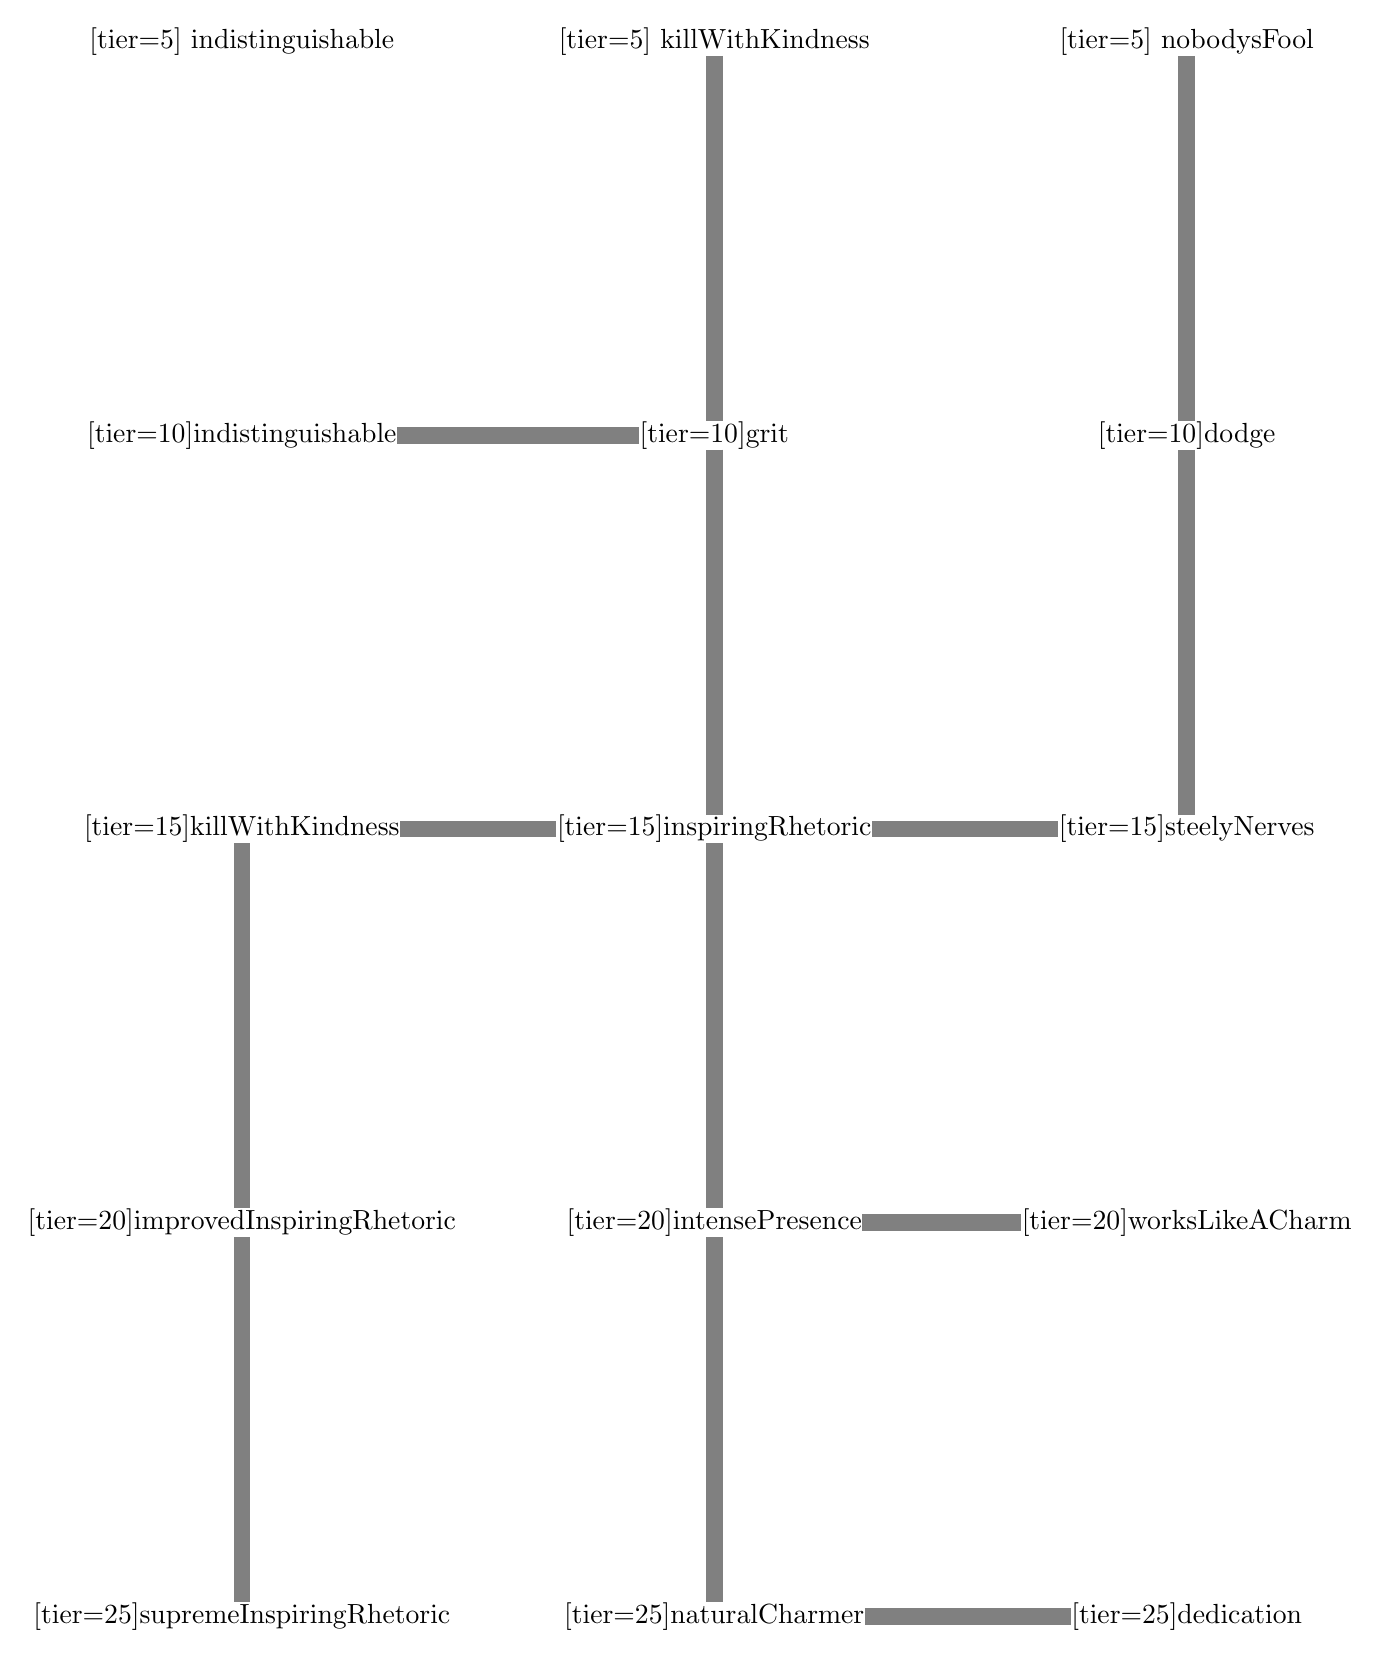
\begin{tikzpicture}
        \draw ( 0,  0) node(aa)[inner sep=0]{\TalentBox[tier=5] {indistinguishable}}
              ( 6,  0) node(ab)[inner sep=0]{\TalentBox[tier=5] {killWithKindness}}
              (12,  0) node(ac)[inner sep=0]{\TalentBox[tier=5] {nobodysFool}}
              ( 0, -5) node(ba)[inner sep=0]{\TalentBox[tier=10]{indistinguishable}}
              ( 6, -5) node(bb)[inner sep=0]{\TalentBox[tier=10]{grit}}
              (12, -5) node(bc)[inner sep=0]{\TalentBox[tier=10]{dodge}}
              ( 0,-10) node(ca)[inner sep=0]{\TalentBox[tier=15]{killWithKindness}}
              ( 6,-10) node(cb)[inner sep=0]{\TalentBox[tier=15]{inspiringRhetoric}}
              (12,-10) node(cc)[inner sep=0]{\TalentBox[tier=15]{steelyNerves}}
              ( 0,-15) node(da)[inner sep=0]{\TalentBox[tier=20]{improvedInspiringRhetoric}}
              ( 6,-15) node(db)[inner sep=0]{\TalentBox[tier=20]{intensePresence}}
              (12,-15) node(dc)[inner sep=0]{\TalentBox[tier=20]{worksLikeACharm}}
              ( 0,-20) node(ea)[inner sep=0]{\TalentBox[tier=25]{supremeInspiringRhetoric}}
              ( 6,-20) node(eb)[inner sep=0]{\TalentBox[tier=25]{naturalCharmer}}
              (12,-20) node(ec)[inner sep=0]{\TalentBox[tier=25]{dedication}}
        ;

        \tikzstyle{bar}=[gray,-,>=stealth, line width=6pt]

        \draw [bar] (ab) to (bb);
        \draw [bar] (ac) to (bc);

        \draw [bar] (bb) to (cb);
        \draw [bar] (bc) to (cc);

        \draw [bar] (ca) to (da);
        \draw [bar] (cb) to (db);

        \draw [bar] (da) to (ea);
        \draw [bar] (db) to (eb);

        \draw [bar] (ba) to (bb);

        \draw [bar] (ca) to (cb);
        \draw [bar] (cb) to (cc);

        \draw [bar] (db) to (dc);

        \draw [bar] (eb) to (ec);
    \end{tikzpicture}
}

\newcommand{\arcanaDescription}{
\section{Arcana}
\epigraph{\textit{
    "So what if the land becomes barren? It’s not like we're going to stick around."
} }{
    Datuu Dawnchaser, Elf Defiler
}

    Athasian wizards drain energy from the surrounding
    soil. The method used labels the wizard as a defiler or a
    preserver. Preservers have the self-control to gather
    energy without destroying plants. Those who do not, or
    who feel no remorse about the damage caused, become
    Defilers. Defilers leave behind sterile soil and infertile ash
    when they cast spells. Because of this, most wastelanders
    blame wizards for the desert landscape that dominates
    the Tablelands today, and their hatred extends to defilers
    and preservers alike. In the seven cities, arcana magic is\\
    outlawed and feared.\\
    Writing is also illegal in the Tablelands, thus wizards
    have to go to great lengths to conceal their spellbooks,
    and they have refined this art to the point where even
    fellow wizards can be hard pressed to identify a spell
    book. When found, they are precious resources, hoarded
    and studied by wizards thirsty for knowledge or power.\\
    \\
    See \nref{tlttree:arcana} for more information.
}

\newcommand{\arcanaTree}{
    \newpage
    \subsection{Arcana Talent Tree}
    \label{tlttree:arcana}

    \textbf{Class Skills:} Arcana, Deception, Alchemy, Vigilance
    \newline

    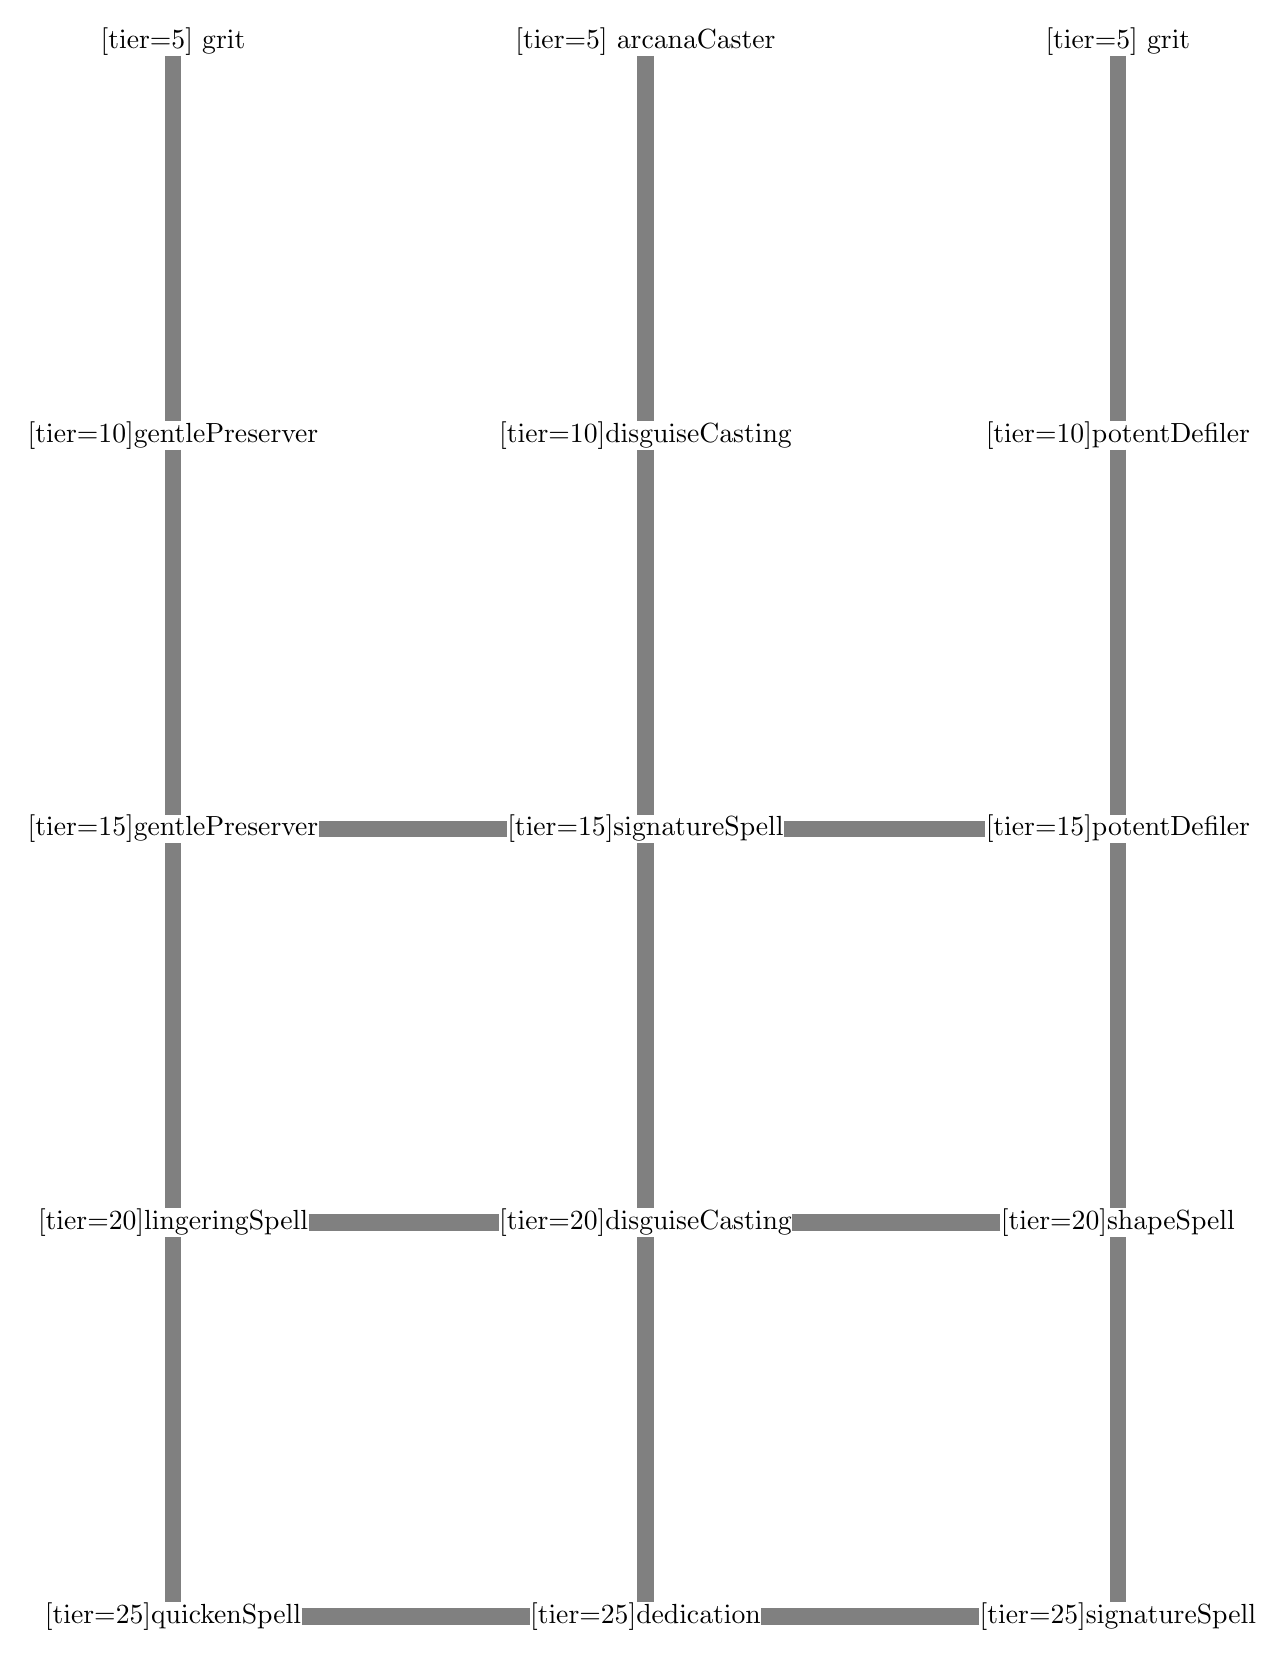
\begin{tikzpicture}
        \draw ( 0,  0) node(aa)[inner sep=0]{\TalentBox[tier=5] {grit}}
              ( 6,  0) node(ab)[inner sep=0]{\TalentBox[tier=5] {arcanaCaster}}
              (12,  0) node(ac)[inner sep=0]{\TalentBox[tier=5] {grit}}
              ( 0, -5) node(ba)[inner sep=0]{\TalentBox[tier=10]{gentlePreserver}}
              ( 6, -5) node(bb)[inner sep=0]{\TalentBox[tier=10]{disguiseCasting}}
              (12, -5) node(bc)[inner sep=0]{\TalentBox[tier=10]{potentDefiler}}
              ( 0,-10) node(ca)[inner sep=0]{\TalentBox[tier=15]{gentlePreserver}}
              ( 6,-10) node(cb)[inner sep=0]{\TalentBox[tier=15]{signatureSpell}}
              (12,-10) node(cc)[inner sep=0]{\TalentBox[tier=15]{potentDefiler}}
              ( 0,-15) node(da)[inner sep=0]{\TalentBox[tier=20]{lingeringSpell}}
              ( 6,-15) node(db)[inner sep=0]{\TalentBox[tier=20]{disguiseCasting}}
              (12,-15) node(dc)[inner sep=0]{\TalentBox[tier=20]{shapeSpell}}
              ( 0,-20) node(ea)[inner sep=0]{\TalentBox[tier=25]{quickenSpell}}
              ( 6,-20) node(eb)[inner sep=0]{\TalentBox[tier=25]{dedication}}
              (12,-20) node(ec)[inner sep=0]{\TalentBox[tier=25]{signatureSpell}}
        ;

        \tikzstyle{bar}=[gray,-,>=stealth, line width=6pt]

        \draw [bar] (aa) edge (ba);
        \draw [bar] (ab) edge (bb);
        \draw [bar] (ac) edge (bc);

        \draw [bar] (ba) edge (ca);
        \draw [bar] (bb) edge (cb);
        \draw [bar] (bc) edge (cc);

        \draw [bar] (ca) edge (da);
        \draw [bar] (cb) edge (db);
        \draw [bar] (cc) edge (dc);

        \draw [bar] (da) edge (ea);
        \draw [bar] (db) edge (eb);
        \draw [bar] (dc) edge (ec);

        \draw [bar] (ca) edge (cb);
        \draw [bar] (cc) edge (cb);

        \draw [bar] (da) edge (db);
        \draw [bar] (dc) edge (db);

        \draw [bar] (ea) edge (eb);
        \draw [bar] (ec) edge (eb);
    \end{tikzpicture}
}

\newcommand{\archerDescription}{
\section{Archer}
    Dedicated to his ranged craft, an archer is often precise and meticules.
    Although he can be a hunter, he can also very well be a noble, shooting only
    in tournaments, rarely setting a foot outside the city walls.
    It goes witout saying that an archer trains with ranged weapons, thus Ranged
    is a career skill. If you can't see your target you surely can't hit it, thus
    an archer is often perceptive. Discipline is needed to for that inner focus
    to hit that tiny spot in the distance. Finally in the heat of the moment, he
    needs to keep his Cool, so that he does not let his projectile fly too early.\\
    \\
    See \nref{tlttree:archer} for more information.
}

\newcommand{\archerTree}{
    \newpage
    \subsection{Archer Talent Tree}
    \label{tlttree:archer}

    \textbf{Class Skills:} Athletics, Cool, Crafting, Perception, Ranged, Discipline
    \newline

    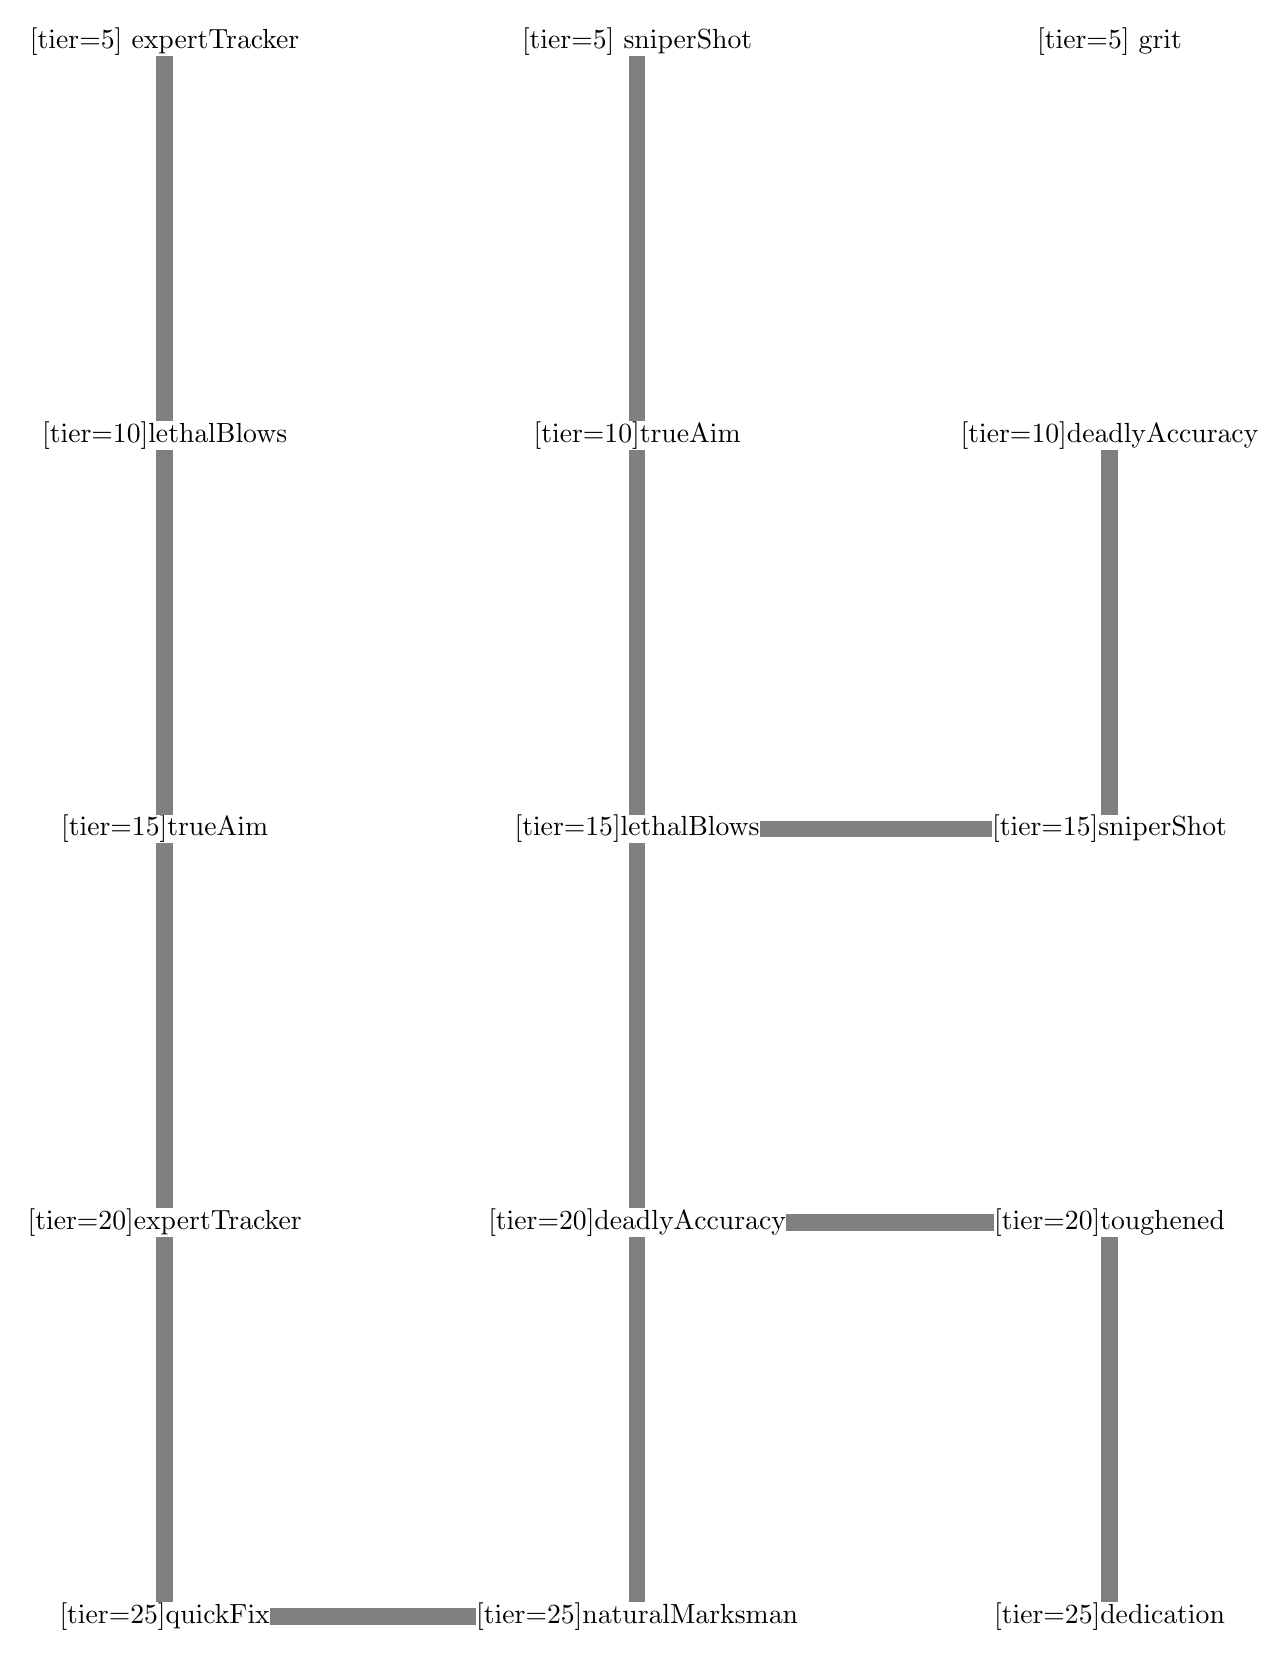
\begin{tikzpicture}
        \draw ( 0,  0) node(aa)[inner sep=0]{\TalentBox[tier=5] {expertTracker}}
              ( 6,  0) node(ab)[inner sep=0]{\TalentBox[tier=5] {sniperShot}}
              (12,  0) node(ac)[inner sep=0]{\TalentBox[tier=5] {grit}}
              ( 0, -5) node(ba)[inner sep=0]{\TalentBox[tier=10]{lethalBlows}}
              ( 6, -5) node(bb)[inner sep=0]{\TalentBox[tier=10]{trueAim}}
              (12, -5) node(bc)[inner sep=0]{\TalentBox[tier=10]{deadlyAccuracy}}
              ( 0,-10) node(ca)[inner sep=0]{\TalentBox[tier=15]{trueAim}}
              ( 6,-10) node(cb)[inner sep=0]{\TalentBox[tier=15]{lethalBlows}}
              (12,-10) node(cc)[inner sep=0]{\TalentBox[tier=15]{sniperShot}}
              ( 0,-15) node(da)[inner sep=0]{\TalentBox[tier=20]{expertTracker}}
              ( 6,-15) node(db)[inner sep=0]{\TalentBox[tier=20]{deadlyAccuracy}}
              (12,-15) node(dc)[inner sep=0]{\TalentBox[tier=20]{toughened}}
              ( 0,-20) node(ea)[inner sep=0]{\TalentBox[tier=25]{quickFix}}
              ( 6,-20) node(eb)[inner sep=0]{\TalentBox[tier=25]{naturalMarksman}}
              (12,-20) node(ec)[inner sep=0]{\TalentBox[tier=25]{dedication}}
        ;

        \tikzstyle{bar}=[gray,-,>=stealth, line width=6pt]

        \draw [bar] (aa) to (ba);
        \draw [bar] (ab) to (bb);

        \draw [bar] (ba) to (ca);
        \draw [bar] (bb) to (cb);
        \draw [bar] (bc) to (cc);

        \draw [bar] (ca) to (da);
        \draw [bar] (cb) to (db);

        \draw [bar] (da) to (ea);
        \draw [bar] (db) to (eb);
        \draw [bar] (dc) to (ec);

        \draw [bar] (cb) to (cc);

        \draw [bar] (db) to (dc);

        \draw [bar] (ea) to (eb);
    \end{tikzpicture}
}

\newcommand{\assassinDescription}{
\section{Assassin}
    \epigraph{\textit{
        \textit{"I live in the darkness, impossible for anyone to see. But when they die, the last person they see is me."}
    } }{
        Listar Bloodhound, Half-Elf Assassin
    }

    Some Description
    \\
    See \nref{tlttree:assassin} for more information.
}


\newcommand{\assassinTree}{
    \newpage
    \subsection{Assassin Talent Tree}
    \label{tlttree:assassin}

    \textbf{Class Skills:} Melee (Light), Perception, Ranged, Knowledge (Underworld), Skulduggery, Stealth
    \newline

    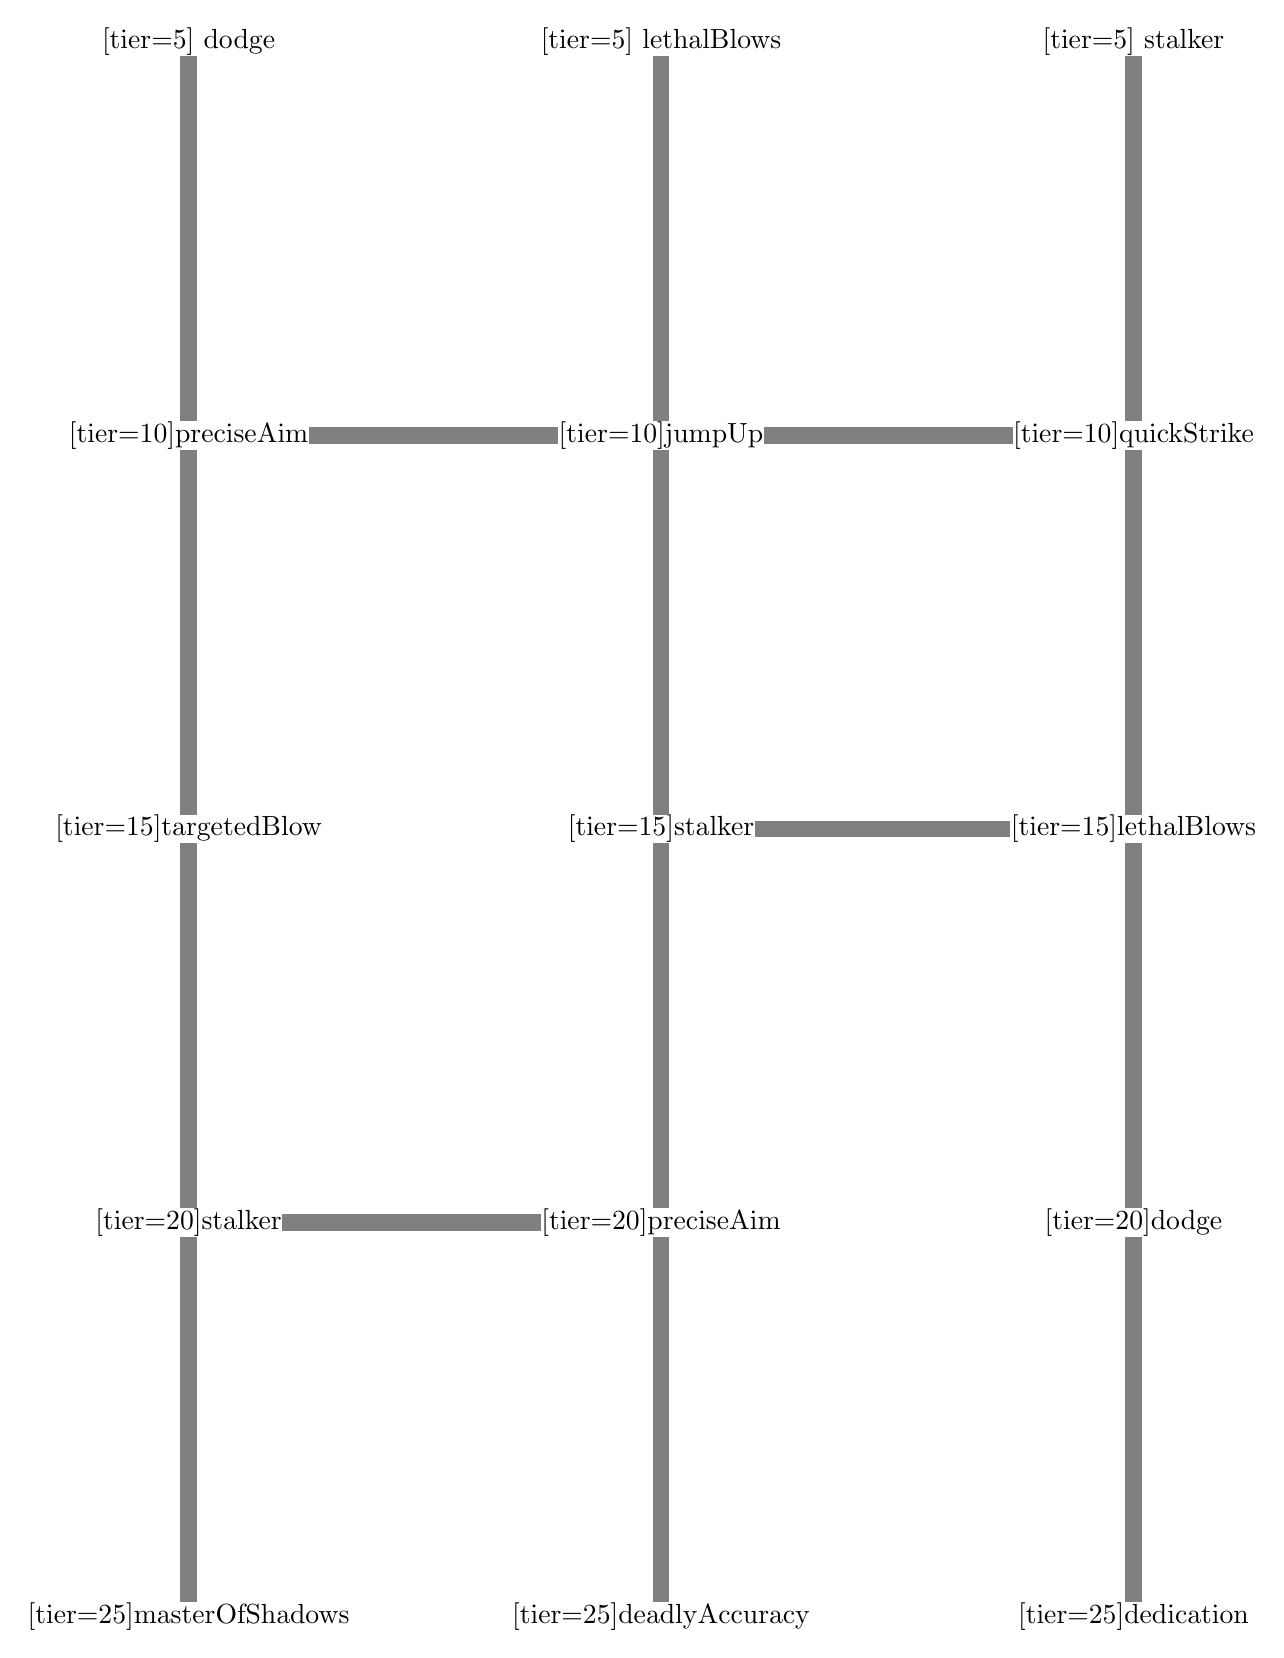
\begin{tikzpicture}
        \draw ( 0,  0) node(aa)[inner sep=0]{\TalentBox[tier=5] {dodge}}
              ( 6,  0) node(ab)[inner sep=0]{\TalentBox[tier=5] {lethalBlows}}
              (12,  0) node(ac)[inner sep=0]{\TalentBox[tier=5] {stalker}}
              ( 0, -5) node(ba)[inner sep=0]{\TalentBox[tier=10]{preciseAim}}
              ( 6, -5) node(bb)[inner sep=0]{\TalentBox[tier=10]{jumpUp}}
              (12, -5) node(bc)[inner sep=0]{\TalentBox[tier=10]{quickStrike}}
              ( 0,-10) node(ca)[inner sep=0]{\TalentBox[tier=15]{targetedBlow}}
              ( 6,-10) node(cb)[inner sep=0]{\TalentBox[tier=15]{stalker}}
              (12,-10) node(cc)[inner sep=0]{\TalentBox[tier=15]{lethalBlows}}
              ( 0,-15) node(da)[inner sep=0]{\TalentBox[tier=20]{stalker}}
              ( 6,-15) node(db)[inner sep=0]{\TalentBox[tier=20]{preciseAim}}
              (12,-15) node(dc)[inner sep=0]{\TalentBox[tier=20]{dodge}}
              ( 0,-20) node(ea)[inner sep=0]{\TalentBox[tier=25]{masterOfShadows}}
              ( 6,-20) node(eb)[inner sep=0]{\TalentBox[tier=25]{deadlyAccuracy}}
              (12,-20) node(ec)[inner sep=0]{\TalentBox[tier=25]{dedication}}
        ;

        \tikzstyle{bar}=[gray,-,>=stealth, line width=6pt]

        \draw [bar] (aa) to (ba);
        \draw [bar] (ab) to (bb);
        \draw [bar] (ac) to (bc);

        \draw [bar] (ba) to (ca);
        \draw [bar] (bb) to (cb);
        \draw [bar] (bc) to (cc);

        \draw [bar] (ca) to (da);
        \draw [bar] (cb) to (db);
        \draw [bar] (cc) to (dc);

        \draw [bar] (da) to (ea);
        \draw [bar] (db) to (eb);
        \draw [bar] (dc) to (ec);

        \draw [bar] (ba) to (bb);
        \draw [bar] (bc) to (bb);

        \draw [bar] (cc) to (cb);

        \draw [bar] (da) to (db);
    \end{tikzpicture}
}

\newcommand{\beastRiderDescription}{
\section{Beast Rider}
\epigraph{\textit{
    "beastRider quote"
} }{
    beastRider quotee
}
    Some Description
    \\
    See \nref{tlttree:beastRider} for more information.
}

\newcommand{\beastRiderTree}{
    \newpage
    \subsection{Beast Rider Talent Tree}
    \label{tlttree:beastRider}

    \textbf{Class Skills:} Athletics, Coordination, Perception, Riding, Survival, Knowledge (Nature)
    \newline

    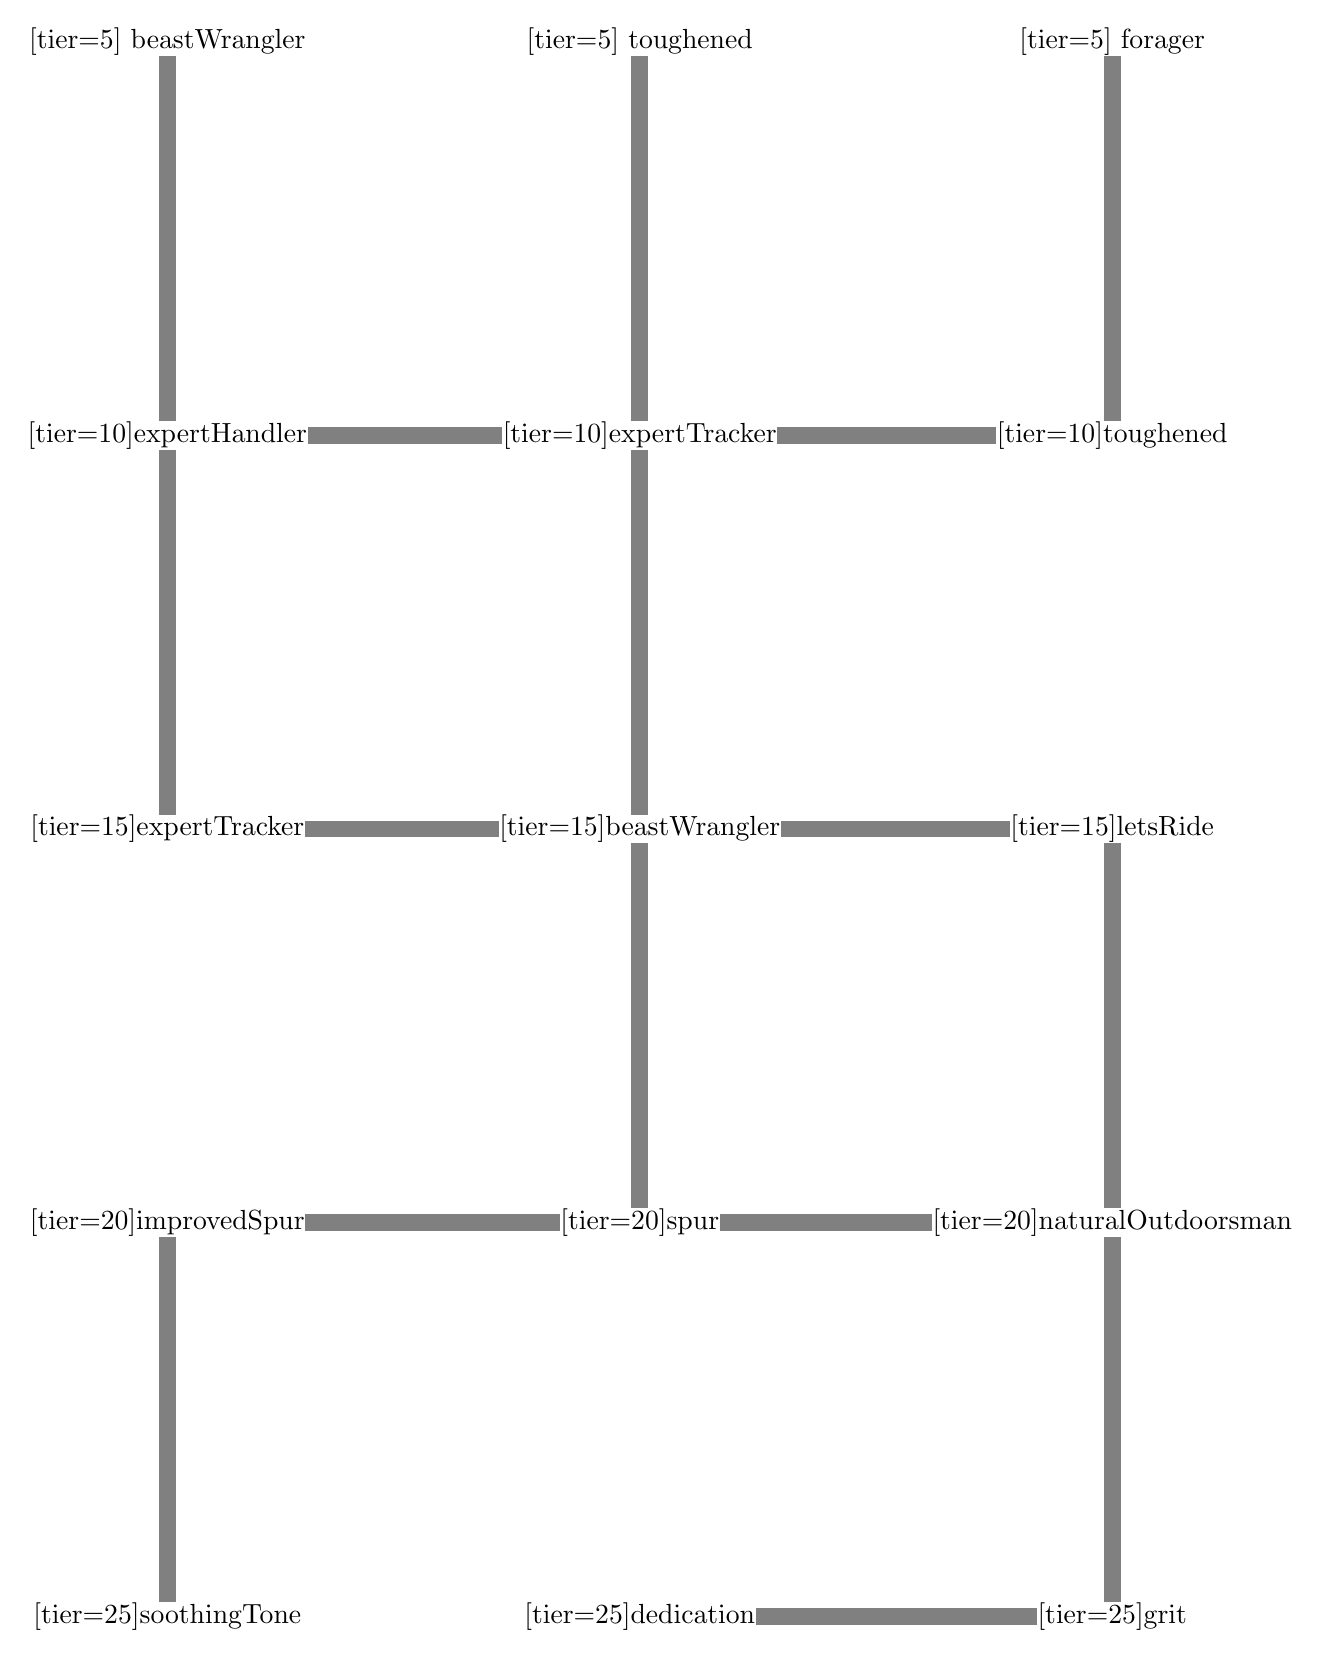
\begin{tikzpicture}
        \draw ( 0,  0) node(aa)[inner sep=0]{\TalentBox[tier=5] {beastWrangler}}
              ( 6,  0) node(ab)[inner sep=0]{\TalentBox[tier=5] {toughened}}
              (12,  0) node(ac)[inner sep=0]{\TalentBox[tier=5] {forager}}
              ( 0, -5) node(ba)[inner sep=0]{\TalentBox[tier=10]{expertHandler}}
              ( 6, -5) node(bb)[inner sep=0]{\TalentBox[tier=10]{expertTracker}}
              (12, -5) node(bc)[inner sep=0]{\TalentBox[tier=10]{toughened}}
              ( 0,-10) node(ca)[inner sep=0]{\TalentBox[tier=15]{expertTracker}}
              ( 6,-10) node(cb)[inner sep=0]{\TalentBox[tier=15]{beastWrangler}}
              (12,-10) node(cc)[inner sep=0]{\TalentBox[tier=15]{letsRide}}
              ( 0,-15) node(da)[inner sep=0]{\TalentBox[tier=20]{improvedSpur}}
              ( 6,-15) node(db)[inner sep=0]{\TalentBox[tier=20]{spur}}
              (12,-15) node(dc)[inner sep=0]{\TalentBox[tier=20]{naturalOutdoorsman}}
              ( 0,-20) node(ea)[inner sep=0]{\TalentBox[tier=25]{soothingTone}}
              ( 6,-20) node(eb)[inner sep=0]{\TalentBox[tier=25]{dedication}}
              (12,-20) node(ec)[inner sep=0]{\TalentBox[tier=25]{grit}}
        ;

        \tikzstyle{bar}=[gray,-,>=stealth, line width=6pt]

        \draw [bar] (aa) to (ba);
        \draw [bar] (ab) to (bb);
        \draw [bar] (ac) to (bc);

        \draw [bar] (ba) to (ca);
        \draw [bar] (bb) to (cb);

        \draw [bar] (cb) to (db);
        \draw [bar] (cc) to (dc);

        \draw [bar] (da) to (ea);
        \draw [bar] (dc) to (ec);

        \draw [bar] (ba) to (bb);
        \draw [bar] (bc) to (bb);

        \draw [bar] (ca) to (cb);
        \draw [bar] (cc) to (cb);

        \draw [bar] (da) to (db);
        \draw [bar] (dc) to (db);

        \draw [bar] (ec) to (eb);
    \end{tikzpicture}
}

%Big Game Hunter
\newcommand{\gameHunterDescription}{
\section{Big Game Hunter}
    Big Game Hunter Text\\
    See \nref{tlttree:gamehunter} for more information.
}

\newcommand{\gameHunterTree}{
    \newpage
    \subsection{Big Game Hunter Talent Tree}
    \label{tlttree:gamehunter}

    \textbf{Class Skills:} Athletics, Knowledge (Nature), Perception, Ranged, Stealth, Survival, 
    \newline

    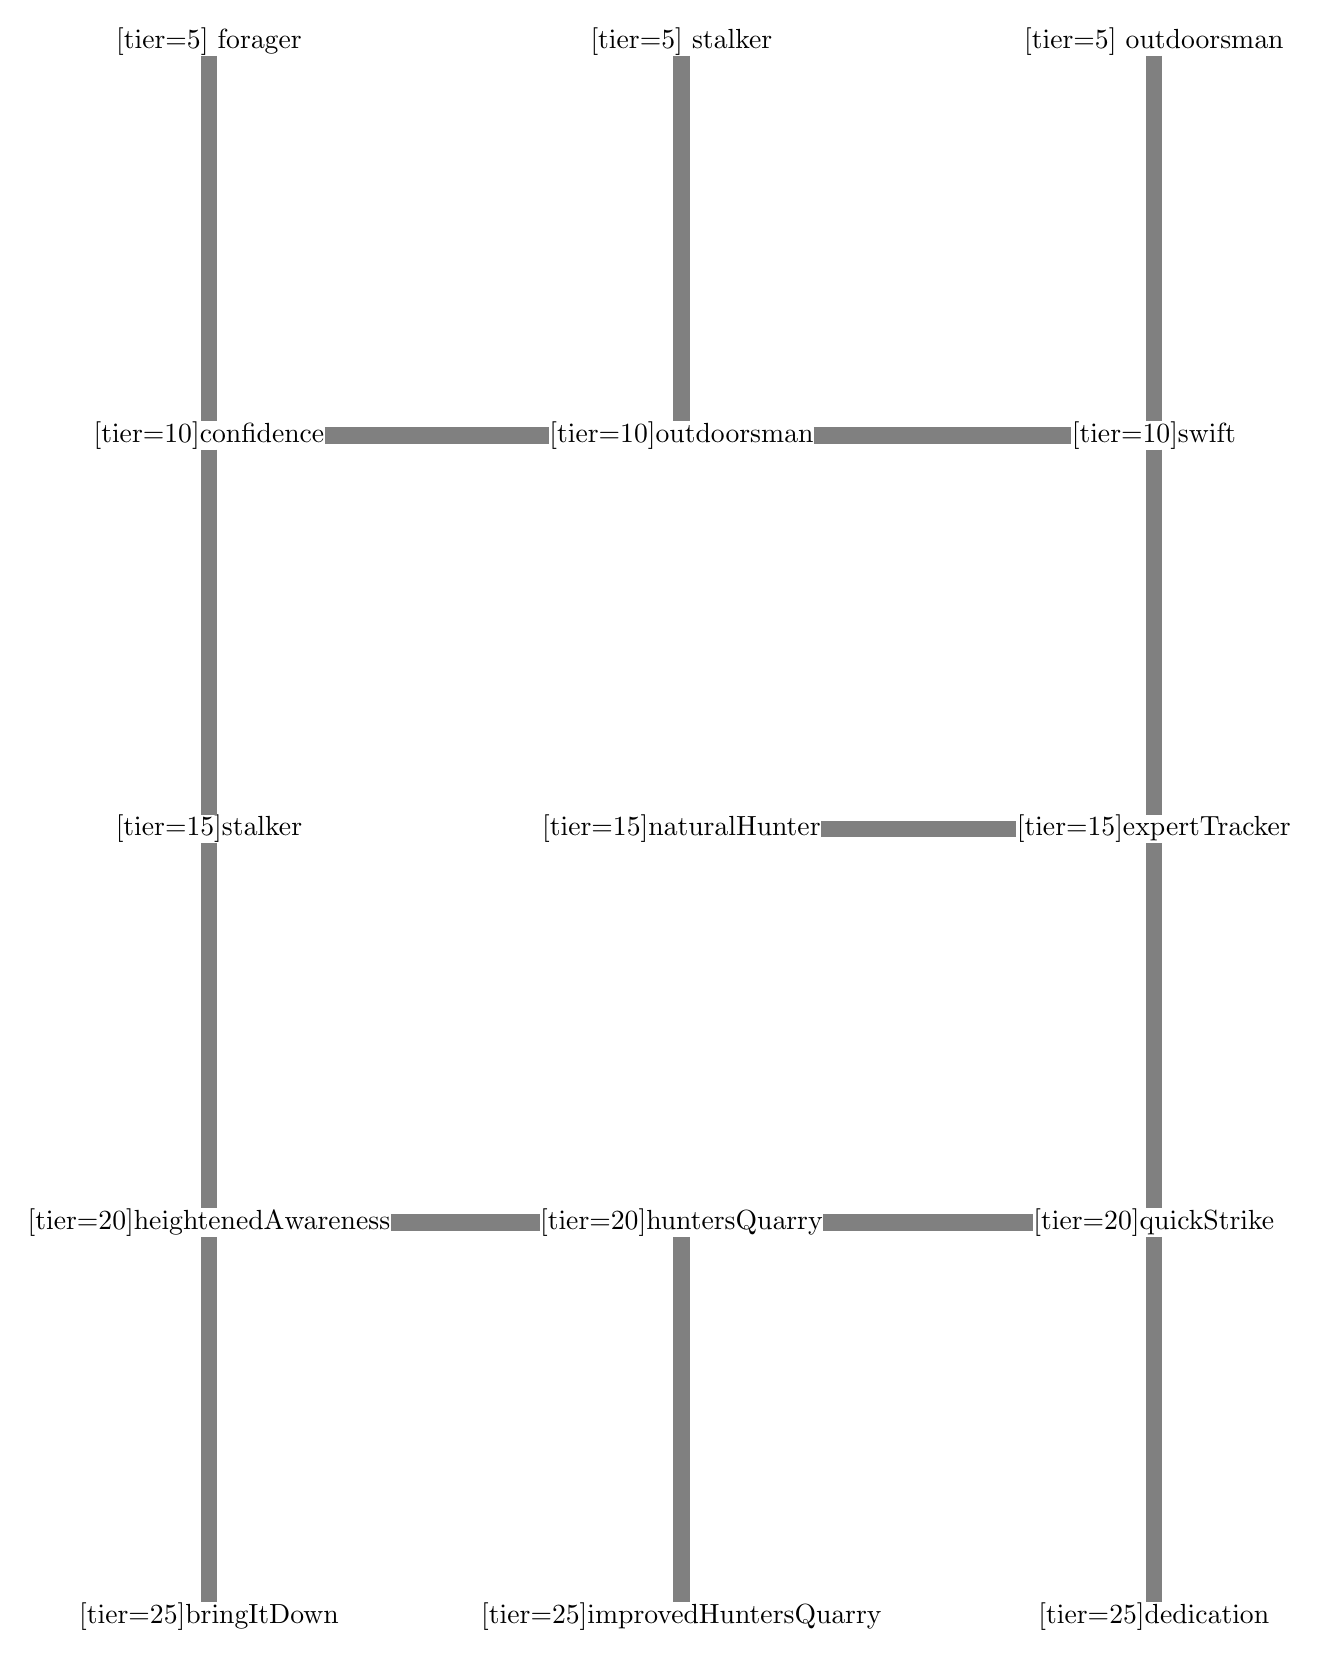
\begin{tikzpicture}
        \draw ( 0,  0) node(aa)[inner sep=0]{\TalentBox[tier=5] {forager}}
              ( 6,  0) node(ab)[inner sep=0]{\TalentBox[tier=5] {stalker}}
              (12,  0) node(ac)[inner sep=0]{\TalentBox[tier=5] {outdoorsman}}
              ( 0, -5) node(ba)[inner sep=0]{\TalentBox[tier=10]{confidence}}
              ( 6, -5) node(bb)[inner sep=0]{\TalentBox[tier=10]{outdoorsman}}
              (12, -5) node(bc)[inner sep=0]{\TalentBox[tier=10]{swift}}
              ( 0,-10) node(ca)[inner sep=0]{\TalentBox[tier=15]{stalker}}
              ( 6,-10) node(cb)[inner sep=0]{\TalentBox[tier=15]{naturalHunter}}
              (12,-10) node(cc)[inner sep=0]{\TalentBox[tier=15]{expertTracker}}
              ( 0,-15) node(da)[inner sep=0]{\TalentBox[tier=20]{heightenedAwareness}}
              ( 6,-15) node(db)[inner sep=0]{\TalentBox[tier=20]{huntersQuarry}}
              (12,-15) node(dc)[inner sep=0]{\TalentBox[tier=20]{quickStrike}}
              ( 0,-20) node(ea)[inner sep=0]{\TalentBox[tier=25]{bringItDown}}
              ( 6,-20) node(eb)[inner sep=0]{\TalentBox[tier=25]{improvedHuntersQuarry}}
              (12,-20) node(ec)[inner sep=0]{\TalentBox[tier=25]{dedication}}
        ;

        \tikzstyle{bar}=[gray,-,>=stealth, line width=6pt]

        \draw [bar] (aa) to (ba);
        \draw [bar] (ab) to (bb);
        \draw [bar] (ac) to (bc);

        \draw [bar] (ba) to (ca);
        \draw [bar] (bc) to (cc);

        \draw [bar] (ca) to (da);
        \draw [bar] (cc) to (dc);

        \draw [bar] (da) to (ea);
        \draw [bar] (db) to (eb);
        \draw [bar] (dc) to (ec);

        \draw [bar] (ba) to (bb);
        \draw [bar] (bb) to (bc);

        \draw [bar] (cb) to (cc);

        \draw [bar] (da) to (db);
        \draw [bar] (db) to (dc);

    \end{tikzpicture}
}

%Vanguard/Bodyguard

\newcommand{\charmerDescription}{
\section{Charmer}
\epigraph{\textit{
    "charmer quote"
} }{
    charmer quotee
}
    Some Description
    \\
    See \nref{tlttree:charmer} for more information.
}

\newcommand{\charmerTree}{
    \newpage
    \subsection{Charmer Talent Tree}
    \label{tlttree:charmer}

    \textbf{Class Skills:} Charm, Cool, Leadership, Negotiation
    \newline

    \begin{tikzpicture}
        \draw ( 0,  0) node[anchor=north east](aa){\TalentBox[tier=5,  width=14em, active=\smoothTalkerActive,              ranked=\smoothTalkerRanked,              name=\smoothTalkerTitle]              {\smoothTalkerDescription}}
              ( 6,  0) node[anchor=north east](ab){\TalentBox[tier=5,  width=14em, active=\inspiringRhetoricActive,         ranked=\inspiringRhetoricRanked,         name=\inspiringRhetoricTitle]         {\inspiringRhetoricDescription}}
              (12,  0) node[anchor=north east](ac){\TalentBox[tier=5,  width=14em, active=\gritActive,                      ranked=\gritRanked,                      name=\gritTitle]                      {\gritDescription}}
              ( 0, -5) node[anchor=north east](ba){\TalentBox[tier=10, width=14em, active=\killWithKindnessActive,          ranked=\killWithKindnessRanked,          name=\killWithKindnessTitle]          {\killWithKindnessDescription}}
              ( 6, -5) node[anchor=north east](bb){\TalentBox[tier=10, width=14em, active=\improvedInspiringRhetoricActive, ranked=\improvedInspiringRhetoricRanked, name=\improvedInspiringRhetoricTitle] {\improvedInspiringRhetoricDescription}}
              (12, -5) node[anchor=north east](bc){\TalentBox[tier=10, width=14em, active=\congenialActive,                 ranked=\congenialRanked,                 name=\congenialTitle]                 {\congenialDescription}}
              ( 0,-10) node[anchor=north east](ca){\TalentBox[tier=15, width=14em, active=\disarmingSmileActive,            ranked=\disarmingSmileRanked,            name=\disarmingSmileTitle]            {\disarmingSmileDescription}}
              ( 6,-10) node[anchor=north east](cb){\TalentBox[tier=15, width=14em, active=\worksLikeACharmActive,           ranked=\worksLikeACharmRanked,           name=\worksLikeACharmTitle]           {\worksLikeACharmDescription}}
              (12,-10) node[anchor=north east](cc){\TalentBox[tier=15, width=14em, active=\disarmingSmileActive,            ranked=\disarmingSmileRanked,            name=\disarmingSmileTitle]            {\disarmingSmileDescription}}
              ( 0,-15) node[anchor=north east](da){\TalentBox[tier=20, width=14em, active=\smoothTalkerActive,              ranked=\smoothTalkerRanked,              name=\smoothTalkerTitle]              {\smoothTalkerDescription}}
              ( 6,-15) node[anchor=north east](db){\TalentBox[tier=20, width=14em, active=\intensePresenceActive,           ranked=\intensePresenceRanked,           name=\intensePresenceTitle]           {\intensePresenceDescription}}
              (12,-15) node[anchor=north east](dc){\TalentBox[tier=20, width=14em, active=\justKiddingActive,               ranked=\justKiddingRanked,               name=\justKiddingTitle]               {\justKiddingDescription}}
              ( 0,-20) node[anchor=north east](ea){\TalentBox[tier=25, width=14em, active=\naturalCharmerActive,            ranked=\naturalCharmerRanked,            name=\naturalCharmerTitle]            {\naturalCharmerDescription}}
              ( 6,-20) node[anchor=north east](eb){\TalentBox[tier=25, width=14em, active=\dedicationActive,                ranked=\dedicationRanked,                name=\dedicationTitle]                {\dedicationDescription}}
              (12,-20) node[anchor=north east](ec){\TalentBox[tier=25, width=14em, active=\dontShootActive,                 ranked=\dontShootRanked,                 name=\dontShootTitle]                 {\dontShootDescription}}
        ;
        \draw [gray,-,>=stealth, line width=6pt] (aa) to (ba);
        \draw [gray,-,>=stealth, line width=6pt] (ab) to (bb);
        \draw [gray,-,>=stealth, line width=6pt] (ac) to (bc);

        \draw [gray,-,>=stealth, line width=6pt] (ba) to (ca);
        \draw [gray,-,>=stealth, line width=6pt] (bc) to (cc);

        \draw [gray,-,>=stealth, line width=6pt] (ca) to (da);
        \draw [gray,-,>=stealth, line width=6pt] (cc) to (dc);

        \draw [gray,-,>=stealth, line width=6pt] (da) to (ea);
        \draw [gray,-,>=stealth, line width=6pt] (dc) to (ec);

        \draw [gray,-,>=stealth, line width=6pt] (bc) to (bb);

        \draw [gray,-,>=stealth, line width=6pt] (cc) to (cb);

        \draw [gray,-,>=stealth, line width=6pt] (da) to (db);
        \draw [gray,-,>=stealth, line width=6pt] (dc) to (db);

        \draw [gray,-,>=stealth, line width=6pt] (ea) to (eb);
        \draw [gray,-,>=stealth, line width=6pt] (ec) to (eb);
    \end{tikzpicture}
}

%Scoundrel

Entrepreneur

\newcommand{\gladiatorDescription}{
\section{Gladiator}
\epigraph{\textit{
    "I might be a slave, but I am famous, I dine well, and my
    company is that of the finest noble women. Tell me, what
    do you have that I do not, slave trader - except the freedom
    to feel miserable?"
} } { Jarek, arena champion }

    The arena is the battlefield of the gladiator. From
    hand-to-hand combat in the mud pits of small forts to the
    grand games of the city-states, the gladiator is a warrior
    who fights to the sounds of people cheering his name or
    cursing his presence. A master of crowd control and the
    art of prolonged combat, gladiators are trained to fight.
    They train to best wild beasts in deadly games for the
    amusement of the masses. They fight for glory, wealth,
    prestige and power. They fight to survive. Some are
    merely slaves, having to fight and perhaps hoping to win
    a chance to obtain freedom, while some fight willingly for
    the thrill of combat or the promise of riches and fame.\\
    \\
    A gladiator often does not have the luxury of choosing her own weapons, and is
    thus familiar with all melee combat skills. Finally she has to be a crowd
    pleaser, for a pure and efficient kill does not attract a full stadium, and
    therefor Charm is a career skill.\\
    \\
    See \nref{tlttree:gladiator} for more information.
}

\newcommand{\gladiatorTree}{
    \newpage
    \subsection{Gladiator Talent Tree}
    \label{tlttree:gladiator}

    \textbf{Class Skills:} Brawl, Melee (Light), Melee (Heavy), Charm
    \newline

    \begin{tikzpicture}
        \draw ( 0,  0) node[anchor=north east](aa){\TalentBox[tier=5,  width=14em, active=\toughenedActive,       ranked=\toughenedRanked,        name=\toughenedTitle]        {\toughenedDescription}}
              ( 6,  0) node[anchor=north east](ab){\TalentBox[tier=5,  width=14em, active=\frenziedAttackActive,  ranked=\frenziedAttackRanked,   name=\frenziedAttackTitle]   {\frenziedAttackDescription}}
              (12,  0) node[anchor=north east](ac){\TalentBox[tier=5,  width=14em, active=\feralStrengthActive,   ranked=\feralStrengthRanked,    name=\feralStrengthTitle]    {\feralStrengthDescription}}
              ( 0, -5) node[anchor=north east](ba){\TalentBox[tier=10, width=14em, active=\feralStrengthActive,   ranked=\feralStrengthRanked,    name=\feralStrengthTitle]    {\feralStrengthDescription}}
              ( 6, -5) node[anchor=north east](bb){\TalentBox[tier=10, width=14em, active=\knockdownActive,       ranked=\knockdownRanked,        name=\knockdownTitle]        {\knockdownDescription}}
              (12, -5) node[anchor=north east](bc){\TalentBox[tier=10, width=14em, active=\heroicFortitudeActive, ranked=\heroicFortitudeRanked,  name=\heroicFortitudeTitle]  {\heroicFortitudeDescription}}
              ( 0,-10) node[anchor=north east](ca){\TalentBox[tier=15, width=14em, active=\hardyActive,           ranked=\hardyRanked,            name=\hardyTitle]            {\hardyDescription}}
              ( 6,-10) node[anchor=north east](cb){\TalentBox[tier=15, width=14em, active=\lethalBlowsActive,     ranked=\lethalBlowsRanked,      name=\lethalBlowsTitle]      {\lethalBlowsDescription}}
              (12,-10) node[anchor=north east](cc){\TalentBox[tier=15, width=14em, active=\toughenedActive,       ranked=\toughenedRanked,        name=\toughenedTitle]        {\toughenedDescription}}
              ( 0,-15) node[anchor=north east](da){\TalentBox[tier=20, width=14em, active=\toughenedActive,       ranked=\toughenedRanked,        name=\toughenedTitle]        {\toughenedDescription}}
              ( 6,-15) node[anchor=north east](db){\TalentBox[tier=20, width=14em, active=\feralStrengthActive,   ranked=\feralStrengthRanked,    name=\feralStrengthTitle]    {\feralStrengthDescription}}
              (12,-15) node[anchor=north east](dc){\TalentBox[tier=20, width=14em, active=\naturalBrawlerActive,  ranked=\naturalBrawlerRanked,   name=\naturalBrawlerTitle]   {\naturalBrawlerDescription}}
              ( 0,-20) node[anchor=north east](ea){\TalentBox[tier=25, width=14em, active=\frenziedAttackActive,  ranked=\frenziedAttackRanked,   name=\frenziedAttackTitle]   {\frenziedAttackDescription}}
              ( 6,-20) node[anchor=north east](eb){\TalentBox[tier=25, width=14em, active=\dedicationActive,      ranked=\dedicationRanked,       name=\dedicationTitle]       {\dedicationDescription}}
              (12,-20) node[anchor=north east](ec){\TalentBox[tier=25, width=14em, active=\defensiveStanceActive, ranked=\defensiveStanceRanked,  name=\defensiveStanceTitle]  {\defensiveStanceDescription}}
        ;
        \draw [gray,-,>=stealth, line width=6pt] (aa) to (ba);
        \draw [gray,-,>=stealth, line width=6pt] (ab) to (bb);
        \draw [gray,-,>=stealth, line width=6pt] (ac) to (bc);
        \draw [gray,-,>=stealth, line width=6pt] (bb) to (cb);
        \draw [gray,-,>=stealth, line width=6pt] (bc) to (cc);
        \draw [gray,-,>=stealth, line width=6pt] (ca) to (da);
        \draw [gray,-,>=stealth, line width=6pt] (db) to (eb);
        \draw [gray,-,>=stealth, line width=6pt] (dc) to (ec);

        \draw [gray,-,>=stealth, line width=6pt] (ba) to (bb);
        \draw [gray,-,>=stealth, line width=6pt] (bc) to (bb);

        \draw [gray,-,>=stealth, line width=6pt] (ca) to (cb);
        \draw [gray,-,>=stealth, line width=6pt] (cc) to (cb);

        \draw [gray,-,>=stealth, line width=6pt] (da) to (db);
        \draw [gray,-,>=stealth, line width=6pt] (dc) to (db);

        \draw [gray,-,>=stealth, line width=6pt] (ea) to (eb);
        \draw [gray,-,>=stealth, line width=6pt] (ec) to (eb);

    \end{tikzpicture}
}

\newcommand{\mercenaryDescription}{
\section{Mercenary}
%\epigraph{\textit{
%    "Mercenary quote"
%} }{
%    Mercenary quotee
%}
%    Some Description
%    \\
    See \nref{tlttree:mercenary} for more information.
}

\newcommand{\mercenaryTree}{
    \newpage
    \subsection{Mercenary Talent Tree}
    \label{tlttree:mercenary}

    \textbf{Class Skills:} Brawl, Coercion, Discipline, Leadership, Melee (Heavy), Melee (Light)
    \newline

    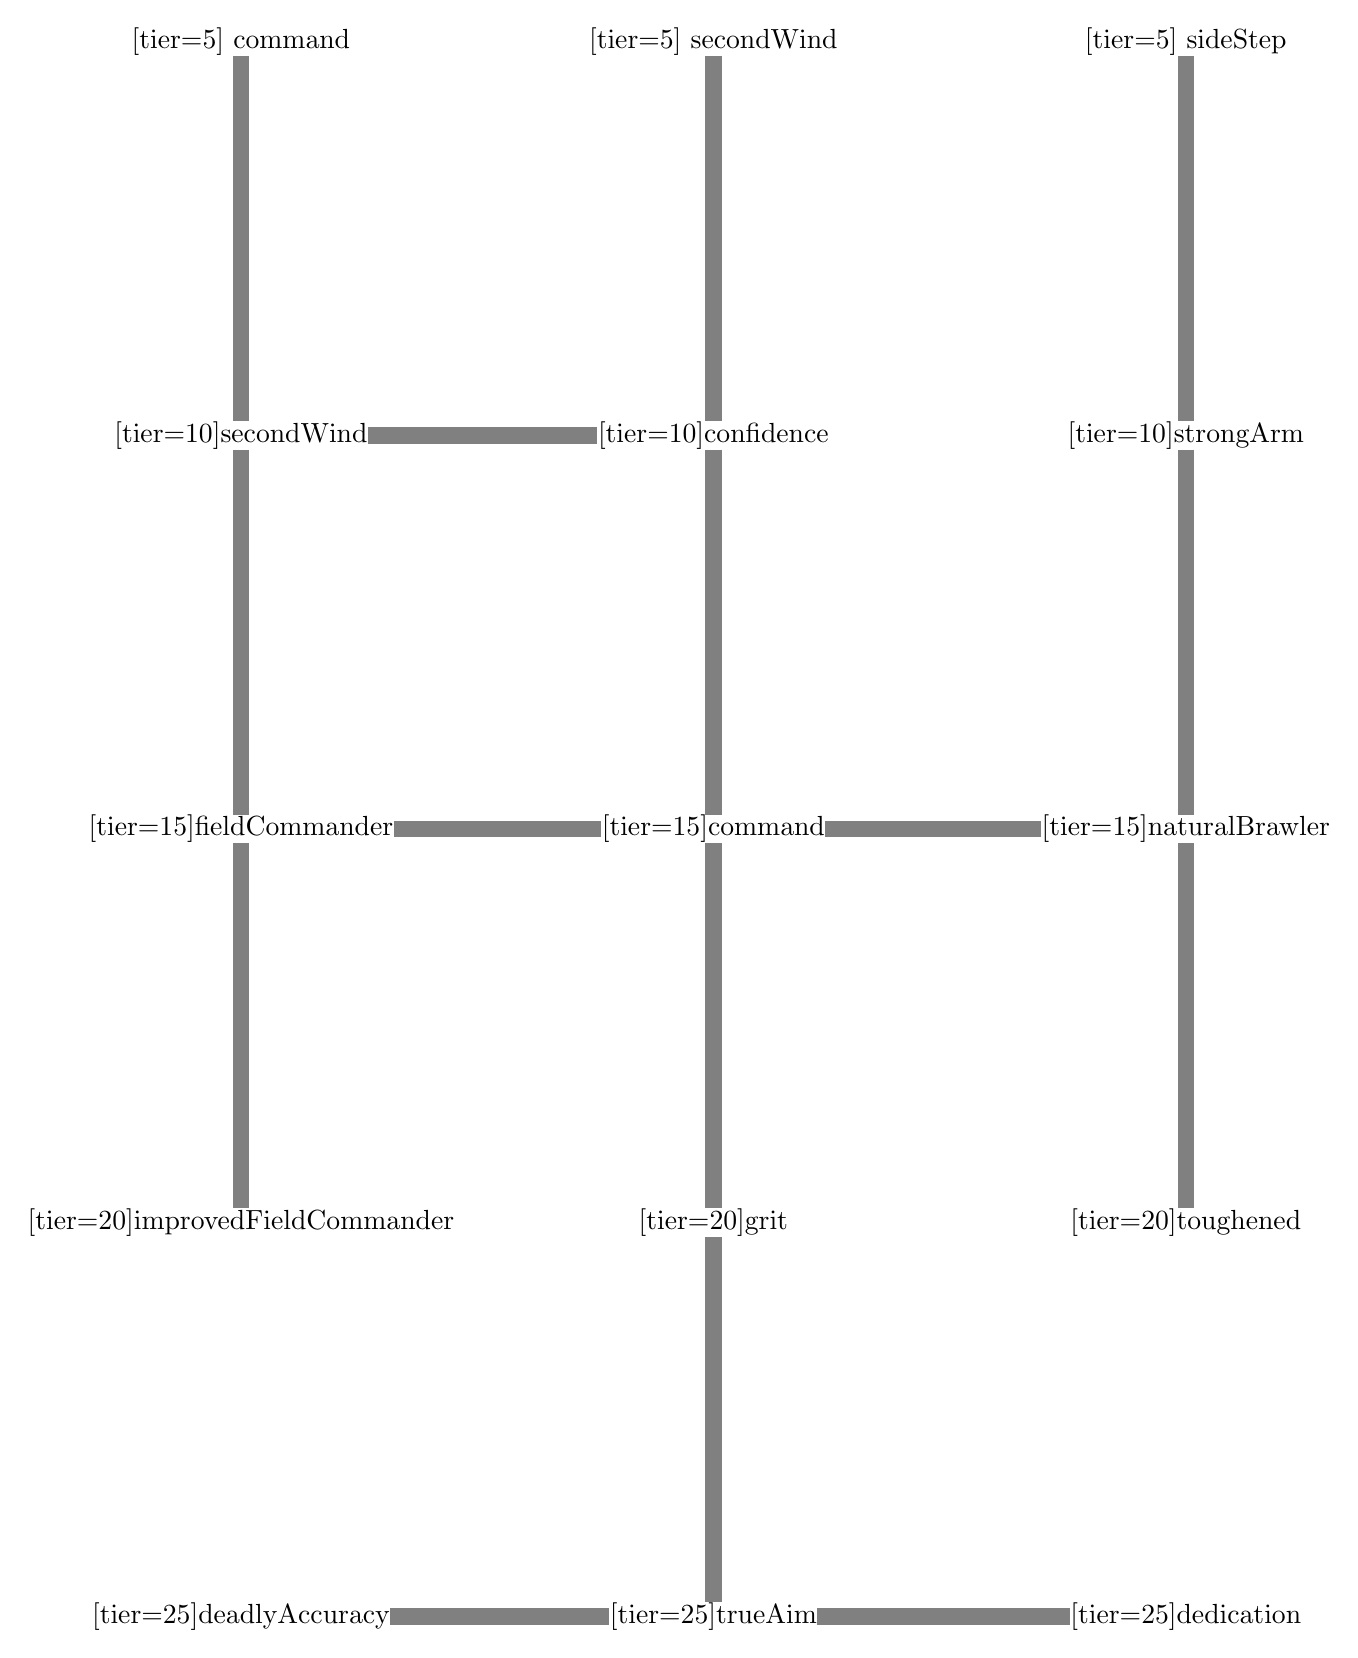
\begin{tikzpicture}
        \draw ( 0,  0) node(aa)[inner sep=0]{\TalentBox[tier=5] {command}}
              ( 6,  0) node(ab)[inner sep=0]{\TalentBox[tier=5] {secondWind}}
              (12,  0) node(ac)[inner sep=0]{\TalentBox[tier=5] {sideStep}}
              ( 0, -5) node(ba)[inner sep=0]{\TalentBox[tier=10]{secondWind}}
              ( 6, -5) node(bb)[inner sep=0]{\TalentBox[tier=10]{confidence}}
              (12, -5) node(bc)[inner sep=0]{\TalentBox[tier=10]{strongArm}}
              ( 0,-10) node(ca)[inner sep=0]{\TalentBox[tier=15]{fieldCommander}}
              ( 6,-10) node(cb)[inner sep=0]{\TalentBox[tier=15]{command}}
              (12,-10) node(cc)[inner sep=0]{\TalentBox[tier=15]{naturalBrawler}}
              ( 0,-15) node(da)[inner sep=0]{\TalentBox[tier=20]{improvedFieldCommander}}
              ( 6,-15) node(db)[inner sep=0]{\TalentBox[tier=20]{grit}}
              (12,-15) node(dc)[inner sep=0]{\TalentBox[tier=20]{toughened}}
              ( 0,-20) node(ea)[inner sep=0]{\TalentBox[tier=25]{deadlyAccuracy}}
              ( 6,-20) node(eb)[inner sep=0]{\TalentBox[tier=25]{trueAim}}
              (12,-20) node(ec)[inner sep=0]{\TalentBox[tier=25]{dedication}}
        ;

        \tikzstyle{bar}=[gray,-,>=stealth, line width=6pt]

        \draw [bar] (aa) to (ba);
        \draw [bar] (ab) to (bb);
        \draw [bar] (ac) to (bc);

        \draw [bar] (ba) to (ca);
        \draw [bar] (bb) to (cb);
        \draw [bar] (bc) to (cc);

        \draw [bar] (ca) to (da);
        \draw [bar] (cb) to (db);
        \draw [bar] (cc) to (dc);

        \draw [bar] (db) to (eb);

        \draw [bar] (ba) to (bb);

        \draw [bar] (ca) to (cb);
        \draw [bar] (cc) to (cb);

        \draw [bar] (ea) to (eb);
        \draw [bar] (ec) to (eb);
    \end{tikzpicture}
}

%%Survivalist
%TODO: reflavor; not really a nomad now
\newcommand{\nomadDescription}{
\section{Nomad}
    Nomad Text\\
    See \nref{tlttree:nomad} for more information.
}

\newcommand{\nomadTree}{
    \newpage
    \subsection{Nomad Talent Tree}
    \label{tlttree:nomad}

    \textbf{Class Skills:} Perception, Resilience, Survival, Knowledge (Nature)
    \newline

    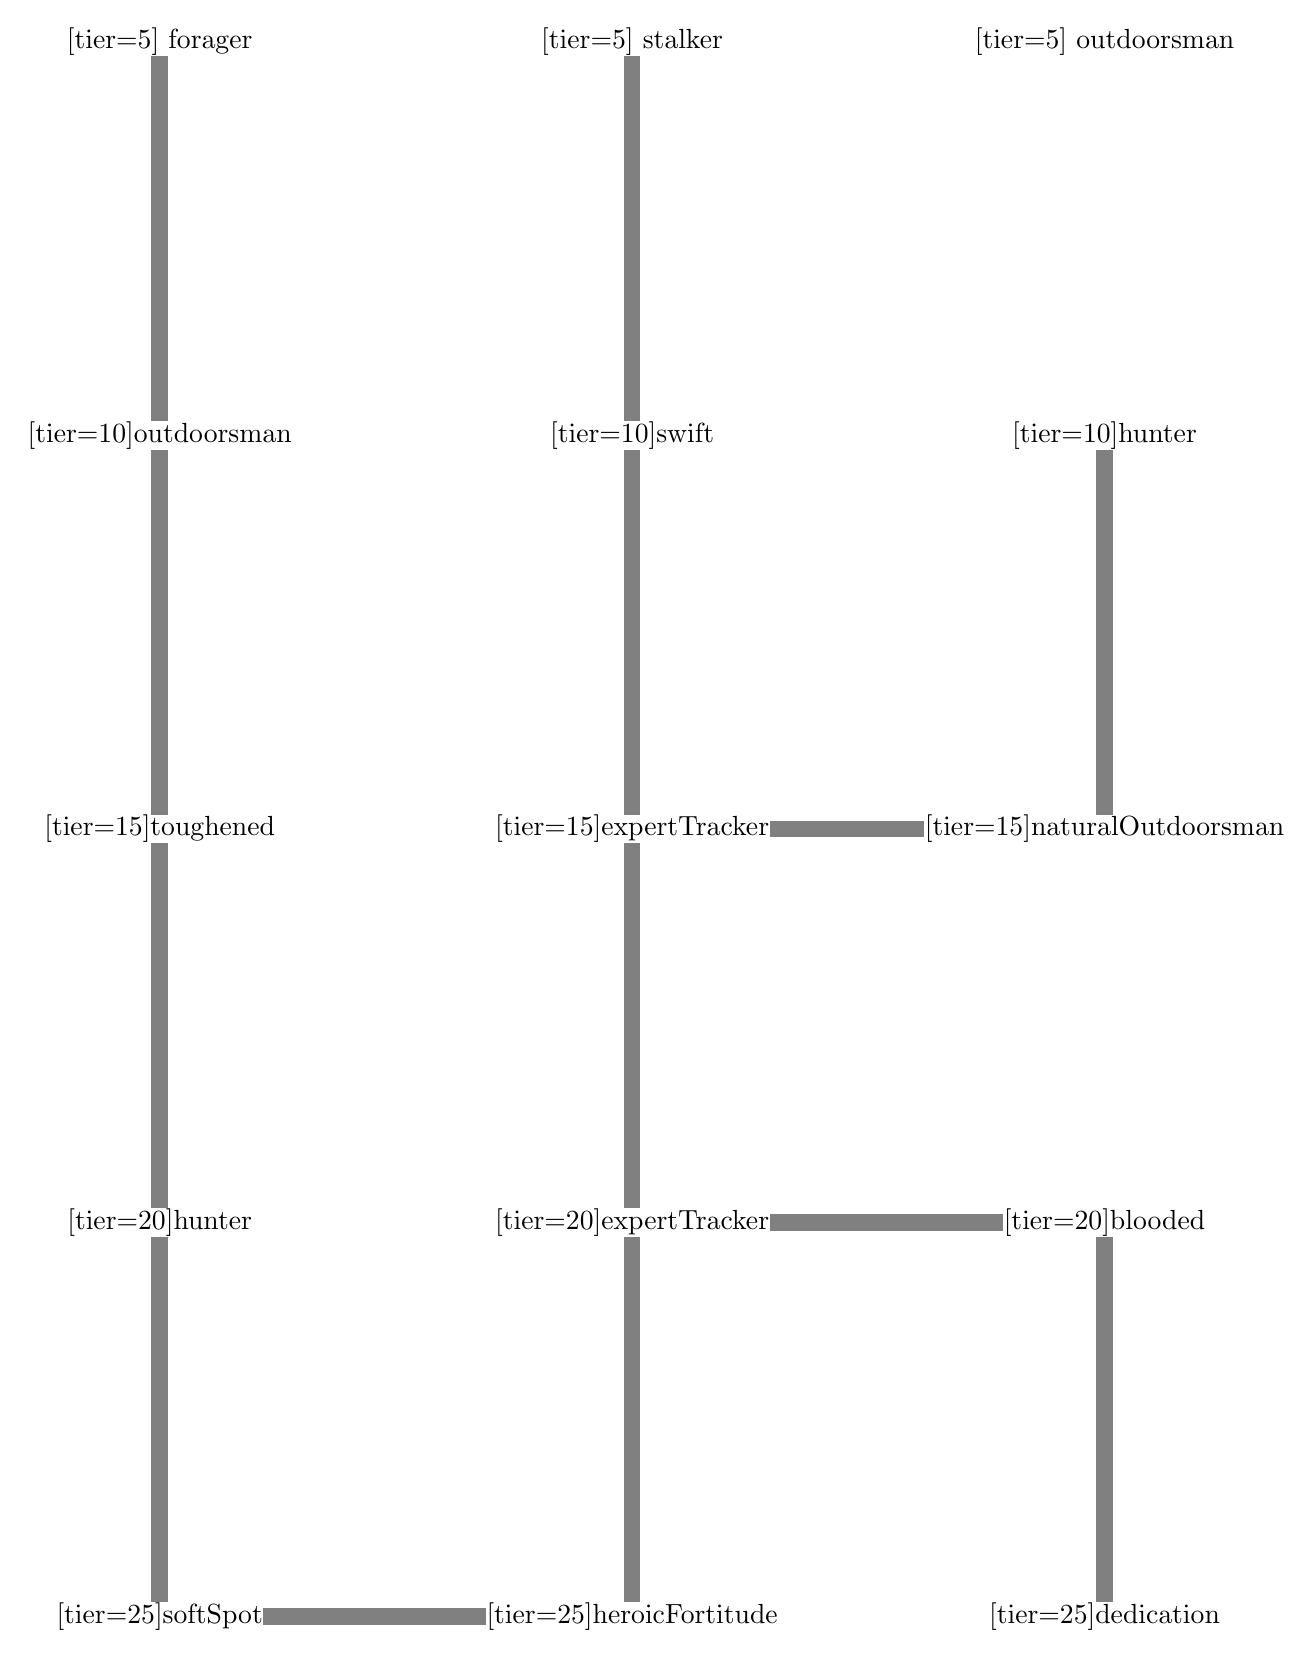
\begin{tikzpicture}
        \draw ( 0,  0) node(aa)[inner sep=0]{\TalentBox[tier=5] {forager}}
              ( 6,  0) node(ab)[inner sep=0]{\TalentBox[tier=5] {stalker}}
              (12,  0) node(ac)[inner sep=0]{\TalentBox[tier=5] {outdoorsman}}
              ( 0, -5) node(ba)[inner sep=0]{\TalentBox[tier=10]{outdoorsman}}
              ( 6, -5) node(bb)[inner sep=0]{\TalentBox[tier=10]{swift}}
              (12, -5) node(bc)[inner sep=0]{\TalentBox[tier=10]{hunter}}
              ( 0,-10) node(ca)[inner sep=0]{\TalentBox[tier=15]{toughened}}
              ( 6,-10) node(cb)[inner sep=0]{\TalentBox[tier=15]{expertTracker}}
              (12,-10) node(cc)[inner sep=0]{\TalentBox[tier=15]{naturalOutdoorsman}}
              ( 0,-15) node(da)[inner sep=0]{\TalentBox[tier=20]{hunter}}
              ( 6,-15) node(db)[inner sep=0]{\TalentBox[tier=20]{expertTracker}}
              (12,-15) node(dc)[inner sep=0]{\TalentBox[tier=20]{blooded}}
              ( 0,-20) node(ea)[inner sep=0]{\TalentBox[tier=25]{softSpot}}
              ( 6,-20) node(eb)[inner sep=0]{\TalentBox[tier=25]{heroicFortitude}}
              (12,-20) node(ec)[inner sep=0]{\TalentBox[tier=25]{dedication}}
        ;

        \tikzstyle{bar}=[gray,-,>=stealth, line width=6pt]

        \draw [bar] (aa) to (ba);
        \draw [bar] (ab) to (bb);

        \draw [bar] (ba) to (ca);
        \draw [bar] (bb) to (cb);
        \draw [bar] (bc) to (cc);

        \draw [bar] (ca) to (da);
        \draw [bar] (cb) to (db);

        \draw [bar] (da) to (ea);
        \draw [bar] (db) to (eb);
        \draw [bar] (dc) to (ec);

        \draw [bar] (cb) to (cc);

        \draw [bar] (db) to (dc);

        \draw [bar] (ea) to (eb);
    \end{tikzpicture}
}

\newcommand{\performerDescription}{
\section{Performer}
\epigraph{\textit{
    "Some people think a club can solve any problem. Unless
    you're a half-giant, there are more sophisticated ways of
    settling a disagreement." } }{ Cabal, half‐elven bard }

    Performers are master the art of entertainment, using their
    performances to amuse nobles and templars and gain wealth.
    Most performers can dazzle a crowd, or incite them to riot.
    Performers tend to learn to play a variety of instruments,
    or recite poetry or old legends by campfire. They can be
    acrobats, performing dazzling displays of physical prowess.\\
    \\
    See \nref{tlttree:performer} for more information.
}

\newcommand{\performerTree}{
    \newpage
    \subsection{Performer Talent Tree}
    \label{tlttree:performer}

    \textbf{Class Skills:} Athletics, Charm, Cool, Coordination, Deception, Streetwise
    \newline

    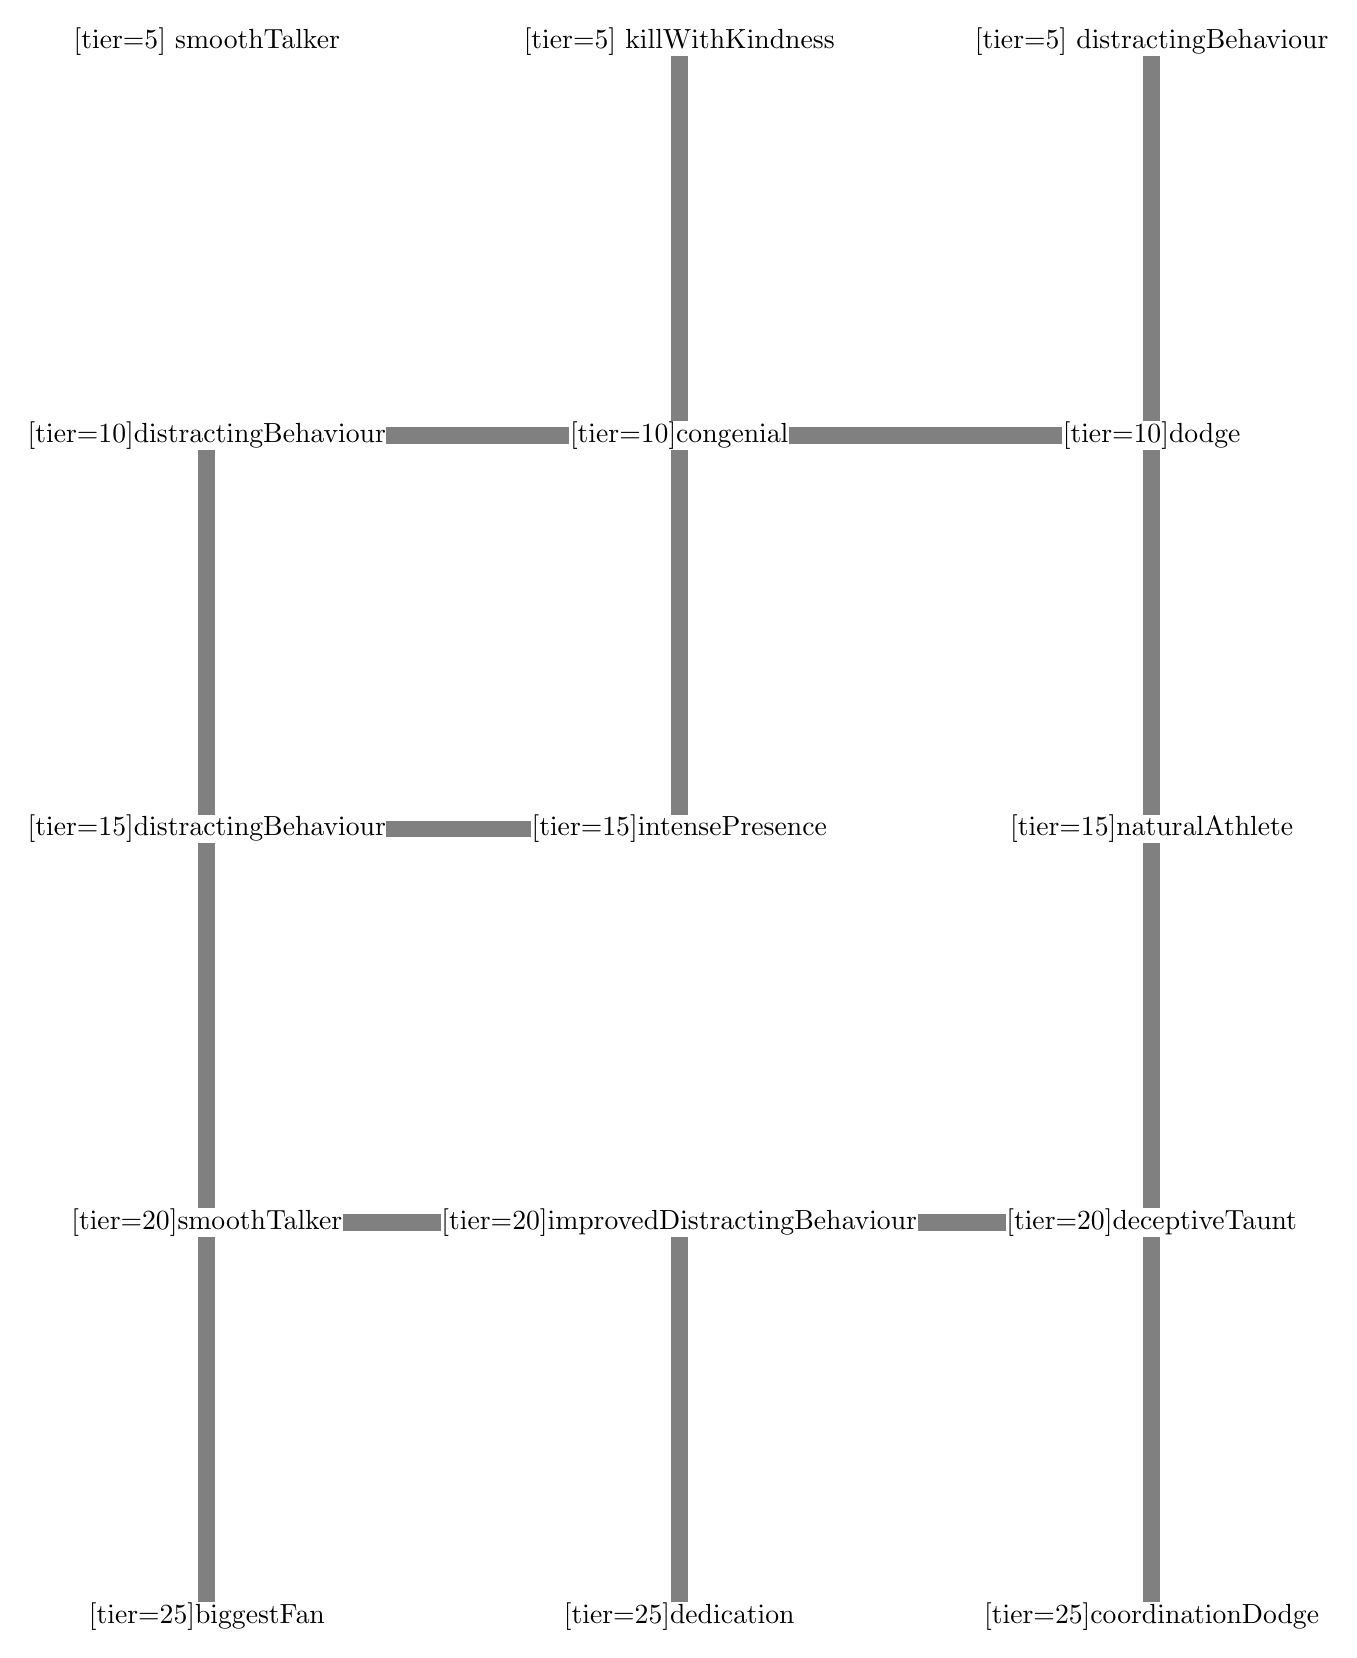
\begin{tikzpicture}
        \draw ( 0,  0) node(aa)[inner sep=0]{\TalentBox[tier=5] {smoothTalker}}
              ( 6,  0) node(ab)[inner sep=0]{\TalentBox[tier=5] {killWithKindness}}
              (12,  0) node(ac)[inner sep=0]{\TalentBox[tier=5] {distractingBehaviour}}
              ( 0, -5) node(ba)[inner sep=0]{\TalentBox[tier=10]{distractingBehaviour}}
              ( 6, -5) node(bb)[inner sep=0]{\TalentBox[tier=10]{congenial}}
              (12, -5) node(bc)[inner sep=0]{\TalentBox[tier=10]{dodge}}
              ( 0,-10) node(ca)[inner sep=0]{\TalentBox[tier=15]{distractingBehaviour}}
              ( 6,-10) node(cb)[inner sep=0]{\TalentBox[tier=15]{intensePresence}}
              (12,-10) node(cc)[inner sep=0]{\TalentBox[tier=15]{naturalAthlete}}
              ( 0,-15) node(da)[inner sep=0]{\TalentBox[tier=20]{smoothTalker}}
              ( 6,-15) node(db)[inner sep=0]{\TalentBox[tier=20]{improvedDistractingBehaviour}}
              (12,-15) node(dc)[inner sep=0]{\TalentBox[tier=20]{deceptiveTaunt}}
              ( 0,-20) node(ea)[inner sep=0]{\TalentBox[tier=25]{biggestFan}}
              ( 6,-20) node(eb)[inner sep=0]{\TalentBox[tier=25]{dedication}}
              (12,-20) node(ec)[inner sep=0]{\TalentBox[tier=25]{coordinationDodge}}
        ;

        \tikzstyle{bar}=[gray,-,>=stealth, line width=6pt]

        \draw [bar] (ab) to (bb);
        \draw [bar] (ac) to (bc);

        \draw [bar] (ba) to (ca);
        \draw [bar] (bb) to (cb);
        \draw [bar] (bc) to (cc);

        \draw [bar] (ca) to (da);
        \draw [bar] (cc) to (dc);

        \draw [bar] (da) to (ea);
        \draw [bar] (db) to (eb);
        \draw [bar] (dc) to (ec);

        \draw [bar] (ba) to (bb);
        \draw [bar] (bc) to (bb);

        \draw [bar] (ca) to (cb);

        \draw [bar] (da) to (db);
        \draw [bar] (dc) to (db);
    \end{tikzpicture}
}

\newcommand{\doctorDescription}{
\section{Healer}
\epigraph{\textit{
    "healer quote"
} }{
    healer quotee
}
    Some Description
    \\
    See \nref{tlttree:doctor} for more information.
}

\newcommand{\doctorTree}{
    \newpage
    \subsection{Healer Talent Tree}
    \label{tlttree:doctor}

    \textbf{Class Skills:} Alchemy, Brawl, Cool, Medicine, Resilience, Knowledge (Education)
    \newline

    
\begin{tikzpicture}
        \draw ( 0,  0) node(aa)[inner sep=0]{\TalentBox[tier=5] {surgeon}}
              ( 6,  0) node(ab)[inner sep=0]{\TalentBox[tier=5] {apothecary}}
              (12,  0) node(ac)[inner sep=0]{\TalentBox[tier=5] {apothecary}}
              ( 0, -5) node(ba)[inner sep=0]{\TalentBox[tier=10]{physician}}
              ( 6, -5) node(bb)[inner sep=0]{\TalentBox[tier=10]{wellRead}}
              (12, -5) node(bc)[inner sep=0]{\TalentBox[tier=10]{surgeon}}
              ( 0,-10) node(ca)[inner sep=0]{\TalentBox[tier=15]{surgeon}}
              ( 6,-10) node(cb)[inner sep=0]{\TalentBox[tier=15]{alchemicalArts}}
              (12,-10) node(cc)[inner sep=0]{\TalentBox[tier=15]{pressurePoint}}
              ( 0,-15) node(da)[inner sep=0]{\TalentBox[tier=20]{physician}}
              ( 6,-15) node(db)[inner sep=0]{\TalentBox[tier=20]{naturalDoctor}}
              (12,-15) node(dc)[inner sep=0]{\TalentBox[tier=20]{anatomyLessons}}
              ( 0,-20) node(ea)[inner sep=0]{\TalentBox[tier=25]{itsNotThatBad}}
              ( 6,-20) node(eb)[inner sep=0]{\TalentBox[tier=25]{masterDoctor}}
              (12,-20) node(ec)[inner sep=0]{\TalentBox[tier=25]{dedication}}
        ;

        \tikzstyle{bar}=[gray,-,>=stealth, line width=6pt]

        \draw [bar] (aa) to (ba);
        \draw [bar] (ab) to (bb);
        \draw [bar] (ac) to (bc);

        \draw [bar] (ba) to (ca);
        \draw [bar] (bb) to (cb);
        \draw [bar] (bc) to (cc);

        \draw [bar] (ca) to (da);
        \draw [bar] (cb) to (db);
        \draw [bar] (cc) to (dc);

        \draw [bar] (da) to (ea);
        \draw [bar] (db) to (eb);
        \draw [bar] (dc) to (ec);

        \draw [bar] (ca) to (cb);
        \draw [bar] (cc) to (cb);

        \draw [bar] (da) to (db);
        \draw [bar] (dc) to (db);

        \draw [bar] (ea) to (eb);
        \draw [bar] (ec) to (eb);
    \end{tikzpicture}
}

\newcommand{\primalDescription}{
\section{Primal}
\epigraph{\textit{
    "A spirit took me in, when neither of my parents would
    accept me. Athas provides for those who care for it. We
    live in a desert simply because no-one cares for the land."
} }{
    Sutura, half‐elven druid
}
    Athasian primal casters, often refered to as druids,
    are the protectors of Athas' dying
    landscape. Patient and often unforgiving, they try to
    preserve and reclaim the barren lands that surround the
    Tyr region. Well armed with spells and abilities from the
    Spirits of the Land, they work to bolster Athas’ failing
    ecology.
    Often, druids prefer to remain hidden, observing the
    behavior of creatures and people before passing
    judgment. Travelers to an oasis are often unaware they
    are being observed; wanton destruction of the oasis will
    find themselves under the full fury of the druid and his
    many abilities.
    \\
    See \nref{tlttree:primal} for more information.
}

\newcommand{\primalTree}{
    \newpage
    \subsection{Primal Talent Tree}
    \label{tlttree:primal}

    \textbf{Class Skills:} Alchemy, Knowledge(Nature), Medicine, Primal, Resilience, Survival
    \newline

    
\begin{tikzpicture}
        \draw ( 0,  0) node(aa)[inner sep=0]{\TalentBox[tier=5] {grit}}
              ( 6,  0) node(ab)[inner sep=0]{\TalentBox[tier=5] {primalCaster}}
              (12,  0) node(ac)[inner sep=0]{\TalentBox[tier=5] {animalCompanion}}
              ( 0, -5) node(ba)[inner sep=0]{\TalentBox[tier=10]{gentlePreserver}}
              ( 6, -5) node(bb)[inner sep=0]{\TalentBox[tier=10]{disguiseCasting}}
              (12, -5) node(bc)[inner sep=0]{\TalentBox[tier=10]{shapeshifter}}
              ( 0,-10) node(ca)[inner sep=0]{\TalentBox[tier=15]{gentlePreserver}}
              ( 6,-10) node(cb)[inner sep=0]{\TalentBox[tier=15]{grit}}
              (12,-10) node(cc)[inner sep=0]{\TalentBox[tier=15]{oneWithNature}}
              ( 0,-15) node(da)[inner sep=0]{\TalentBox[tier=20]{gentlePreserver}}
              ( 6,-15) node(db)[inner sep=0]{\TalentBox[tier=20]{disguiseCasting}}
              (12,-15) node(dc)[inner sep=0]{\TalentBox[tier=20]{shapeshifter}}
              ( 0,-20) node(ea)[inner sep=0]{\TalentBox[tier=25]{quickenSpell}}
              ( 6,-20) node(eb)[inner sep=0]{\TalentBox[tier=25]{dedication}}
              (12,-20) node(ec)[inner sep=0]{\TalentBox[tier=25]{shapeshifter}}
        ;

        \tikzstyle{bar}=[gray,-,>=stealth, line width=6pt]

        \draw [bar] (aa) to (ba);
        \draw [bar] (ab) to (bb);
        \draw [bar] (ac) to (bc);

        \draw [bar] (ba) to (ca);
        \draw [bar] (bb) to (cb);
        \draw [bar] (bc) to (cc);

        \draw [bar] (ca) to (da);
        \draw [bar] (cb) to (db);
        \draw [bar] (cc) to (dc);

        \draw [bar] (da) to (ea);
        \draw [bar] (db) to (eb);
        \draw [bar] (dc) to (ec);

        \draw [bar] (ca) to (cb);

        \draw [bar] (da) to (db);

        \draw [bar] (ea) to (eb);
        \draw [bar] (ec) to (eb);
    \end{tikzpicture}
}

\newcommand{\psionDescription}{
\section{Psion}
\epigraph{\textit{
    "Resist all you like. I have ways of making you think." } }{ Dechares, Dwarven inquisitor }

    The psion learns the Way, a philosophy of mental
    discipline, to become master of his will, or innate mental
    power. Most aspiring psions seek out an instructor, a
    master of the Way. Most Athasian cities contain psionic
    academies where students receive instructions in
    exchange for money or loyal service.\\
    \\
    See \nref{tlttree:psion} for more information.
}

\newcommand{\psionTree}{
    \newpage
    \subsection{Psion Talent Tree}
    \label{tlttree:psion}

    \textbf{Class Skills:} Cool, Psionics, Perception, Vigilance, Discipline, Resilience
    \newline

    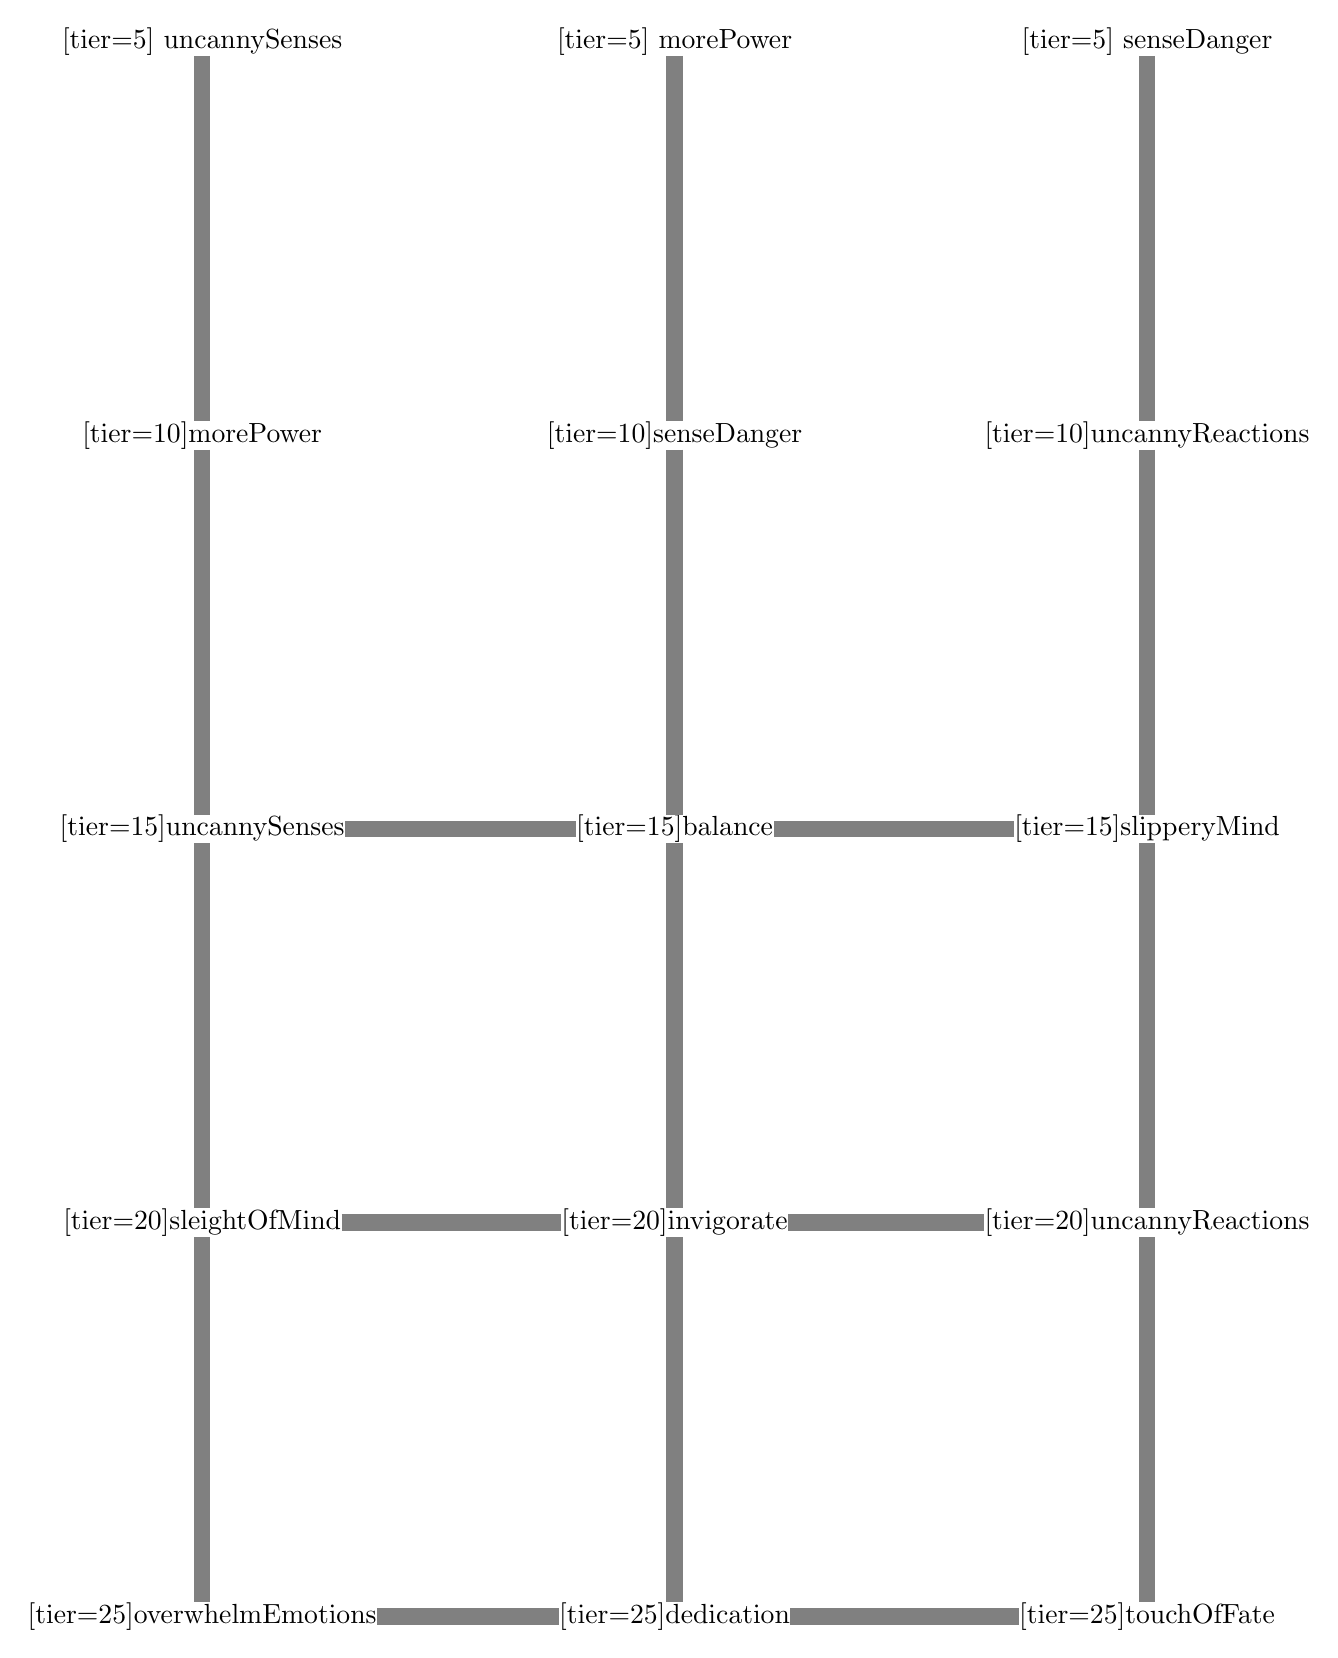
\begin{tikzpicture}
        \draw ( 0,  0) node(aa)[inner sep=0]{\TalentBox[tier=5] {uncannySenses}}
              ( 6,  0) node(ab)[inner sep=0]{\TalentBox[tier=5] {morePower}}
              (12,  0) node(ac)[inner sep=0]{\TalentBox[tier=5] {senseDanger}}
              ( 0, -5) node(ba)[inner sep=0]{\TalentBox[tier=10]{morePower}}
              ( 6, -5) node(bb)[inner sep=0]{\TalentBox[tier=10]{senseDanger}}
              (12, -5) node(bc)[inner sep=0]{\TalentBox[tier=10]{uncannyReactions}}
              ( 0,-10) node(ca)[inner sep=0]{\TalentBox[tier=15]{uncannySenses}}
              ( 6,-10) node(cb)[inner sep=0]{\TalentBox[tier=15]{balance}}
              (12,-10) node(cc)[inner sep=0]{\TalentBox[tier=15]{slipperyMind}}
              ( 0,-15) node(da)[inner sep=0]{\TalentBox[tier=20]{sleightOfMind}}
              ( 6,-15) node(db)[inner sep=0]{\TalentBox[tier=20]{invigorate}}
              (12,-15) node(dc)[inner sep=0]{\TalentBox[tier=20]{uncannyReactions}}
              ( 0,-20) node(ea)[inner sep=0]{\TalentBox[tier=25]{overwhelmEmotions}}
              ( 6,-20) node(eb)[inner sep=0]{\TalentBox[tier=25]{dedication}}
              (12,-20) node(ec)[inner sep=0]{\TalentBox[tier=25]{touchOfFate}}
        ;

        \tikzstyle{bar}=[gray,-,>=stealth, line width=6pt]

        \draw [bar] (aa) to (ba);
        \draw [bar] (ab) to (bb);
        \draw [bar] (ac) to (bc);

        \draw [bar] (ba) to (ca);
        \draw [bar] (bb) to (cb);
        \draw [bar] (bc) to (cc);

        \draw [bar] (ca) to (da);
        \draw [bar] (cb) to (db);
        \draw [bar] (cc) to (dc);

        \draw [bar] (da) to (ea);
        \draw [bar] (db) to (eb);
        \draw [bar] (dc) to (ec);

        \draw [bar] (ca) to (cb);
        \draw [bar] (cc) to (cb);

        \draw [bar] (da) to (db);
        \draw [bar] (dc) to (db);

        \draw [bar] (ea) to (eb);
        \draw [bar] (ec) to (eb);
    \end{tikzpicture}
}

%%Trailblazer
\newcommand{\raiderDescription}{
\section{Raider}
    Raider Text\\
    See \nref{tlttree:raider} for more information.
}

\newcommand{\raiderTree}{
    \newpage
    \subsection{Raider Talent Tree}
    \label{tlttree:raider}

    \textbf{Class Skills:} Brawl, Cool, Coorcion, Perception, Ranged, Discipline
    \newline

    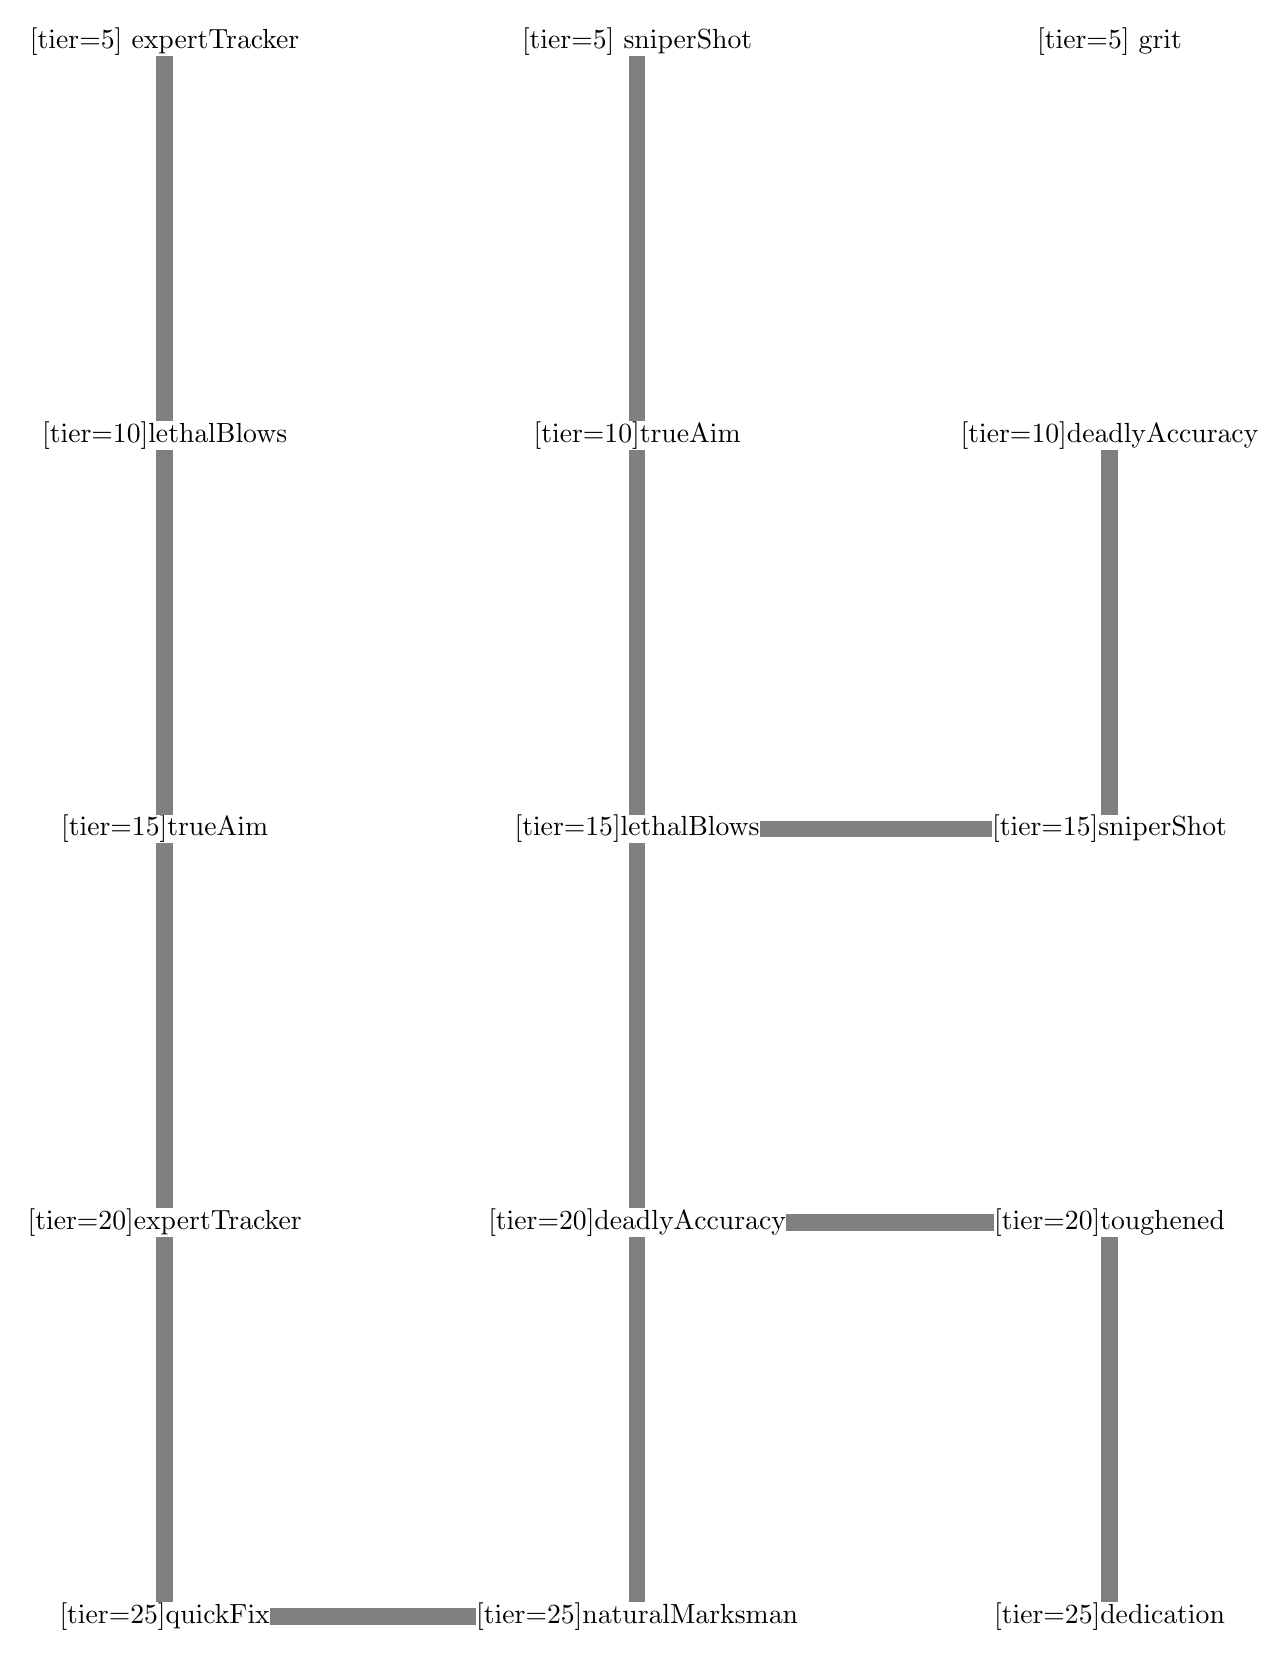
\begin{tikzpicture}
        \draw ( 0,  0) node(aa)[inner sep=0]{\TalentBox[tier=5] {expertTracker}}
              ( 6,  0) node(ab)[inner sep=0]{\TalentBox[tier=5] {sniperShot}}
              (12,  0) node(ac)[inner sep=0]{\TalentBox[tier=5] {grit}}
              ( 0, -5) node(ba)[inner sep=0]{\TalentBox[tier=10]{lethalBlows}}
              ( 6, -5) node(bb)[inner sep=0]{\TalentBox[tier=10]{trueAim}}
              (12, -5) node(bc)[inner sep=0]{\TalentBox[tier=10]{deadlyAccuracy}}
              ( 0,-10) node(ca)[inner sep=0]{\TalentBox[tier=15]{trueAim}}
              ( 6,-10) node(cb)[inner sep=0]{\TalentBox[tier=15]{lethalBlows}}
              (12,-10) node(cc)[inner sep=0]{\TalentBox[tier=15]{sniperShot}}
              ( 0,-15) node(da)[inner sep=0]{\TalentBox[tier=20]{expertTracker}}
              ( 6,-15) node(db)[inner sep=0]{\TalentBox[tier=20]{deadlyAccuracy}}
              (12,-15) node(dc)[inner sep=0]{\TalentBox[tier=20]{toughened}}
              ( 0,-20) node(ea)[inner sep=0]{\TalentBox[tier=25]{quickFix}}
              ( 6,-20) node(eb)[inner sep=0]{\TalentBox[tier=25]{naturalMarksman}}
              (12,-20) node(ec)[inner sep=0]{\TalentBox[tier=25]{dedication}}
        ;

        \tikzstyle{bar}=[gray,-,>=stealth, line width=6pt]

        \draw [bar] (aa) to (ba);
        \draw [bar] (ab) to (bb);

        \draw [bar] (ba) to (ca);
        \draw [bar] (bb) to (cb);
        \draw [bar] (bc) to (cc);

        \draw [bar] (ca) to (da);
        \draw [bar] (cb) to (db);

        \draw [bar] (da) to (ea);
        \draw [bar] (db) to (eb);
        \draw [bar] (dc) to (ec);

        \draw [bar] (cb) to (cc);

        \draw [bar] (db) to (dc);

        \draw [bar] (ea) to (eb);
    \end{tikzpicture}
}

%Scholar
\newcommand{\scholarDescription}{
\section{Scholar}
    Scholar text
    See \nref{tlttree:scholar} for more information.
}

\newcommand{\scholarTree}{
    \newpage
    \subsection{Scholar Talent Tree}
    \label{tlttree:scholar}

    \textbf{Class Skills:} Discipline, Perception, Knowledge (Education), Knowledge (Geography), Knowledge (Nature), Knowledge (Underworld)
    \newline

    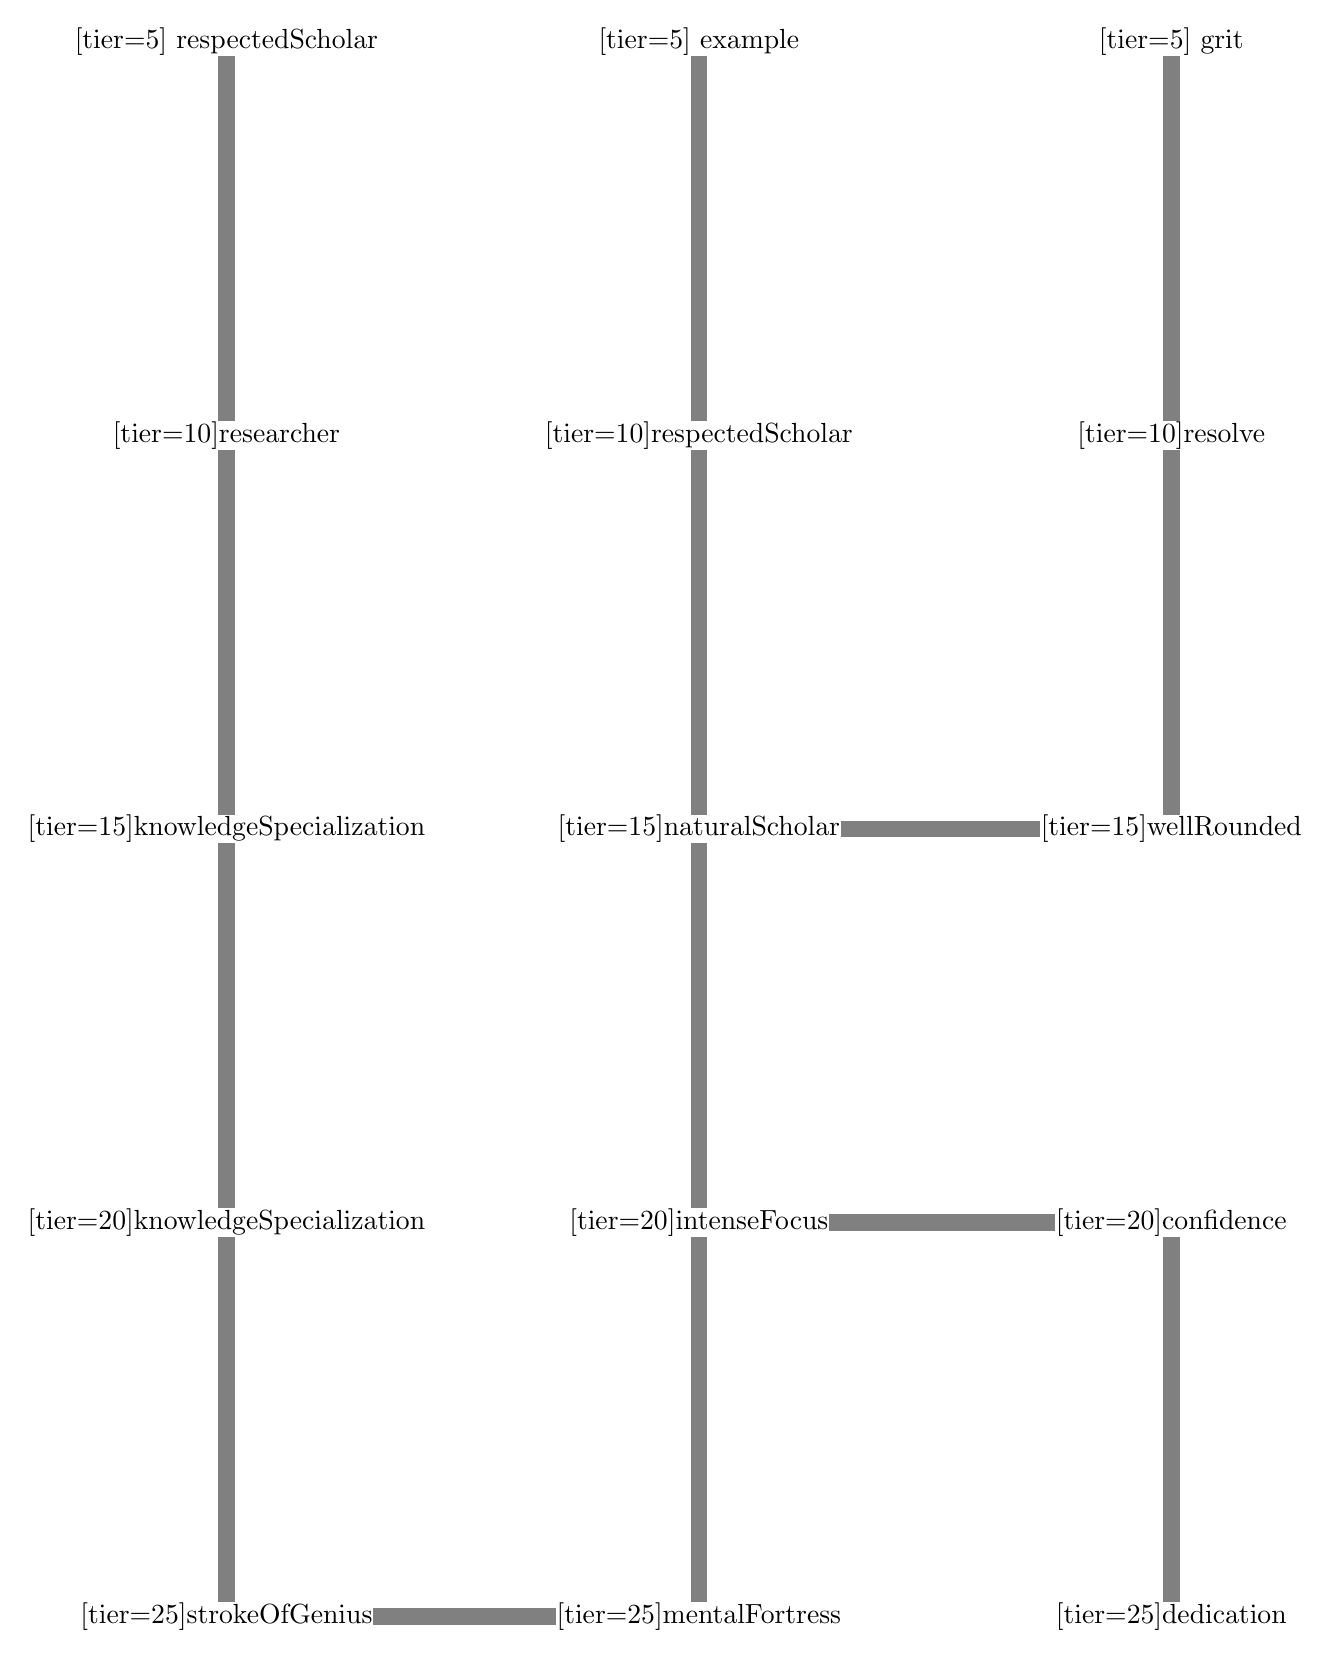
\begin{tikzpicture}
        \draw ( 0,  0) node(aa)[inner sep=0]{\TalentBox[tier=5] {respectedScholar}}
              ( 6,  0) node(ab)[inner sep=0]{\TalentBox[tier=5] {example}}
              (12,  0) node(ac)[inner sep=0]{\TalentBox[tier=5] {grit}}
              ( 0, -5) node(ba)[inner sep=0]{\TalentBox[tier=10]{researcher}}
              ( 6, -5) node(bb)[inner sep=0]{\TalentBox[tier=10]{respectedScholar}}
              (12, -5) node(bc)[inner sep=0]{\TalentBox[tier=10]{resolve}}
              ( 0,-10) node(ca)[inner sep=0]{\TalentBox[tier=15]{knowledgeSpecialization}}
              ( 6,-10) node(cb)[inner sep=0]{\TalentBox[tier=15]{naturalScholar}}
              (12,-10) node(cc)[inner sep=0]{\TalentBox[tier=15]{wellRounded}}
              ( 0,-15) node(da)[inner sep=0]{\TalentBox[tier=20]{knowledgeSpecialization}}
              ( 6,-15) node(db)[inner sep=0]{\TalentBox[tier=20]{intenseFocus}}
              (12,-15) node(dc)[inner sep=0]{\TalentBox[tier=20]{confidence}}
              ( 0,-20) node(ea)[inner sep=0]{\TalentBox[tier=25]{strokeOfGenius}}
              ( 6,-20) node(eb)[inner sep=0]{\TalentBox[tier=25]{mentalFortress}}
              (12,-20) node(ec)[inner sep=0]{\TalentBox[tier=25]{dedication}}
        ;

        \tikzstyle{bar}=[gray,-,>=stealth, line width=6pt]

        \draw [bar] (aa) to (ba);
        \draw [bar] (ab) to (bb);
        \draw [bar] (ac) to (bc);

        \draw [bar] (ba) to (ca);
        \draw [bar] (bb) to (cb);
        \draw [bar] (bc) to (cc);

        \draw [bar] (ca) to (da);
        \draw [bar] (cb) to (db);

        \draw [bar] (da) to (ea);
        \draw [bar] (db) to (eb);
        \draw [bar] (dc) to (ec);

        \draw [bar] (cb) to (cc);

        \draw [bar] (db) to (dc);

        \draw [bar] (ea) to (eb);
    \end{tikzpicture}
}

Survivalist

%Clairsentience
Clairsentience powers enable a character to learn secrets long forgotten, to
glimpse the immediate future and predict the far future, to find hidden
objects, and to know what is normally unknowable. A psion who specializes
in clairsentience is known as a seer, and is most akin to an arcane diviner.
In 3rd edition, Clairsentience is linked to Wisdom.

Seek
Farsight

\newcommand{\thiefDescription}{
\section{Thief}
    \epigraph{\textit{"Marek, always helpful, said that the UnderTyr
    catacombs are supposed to be haunted. Think I'll go make
    some inquiries about where a 'heretic' like me can get some
    holy earth. Always go prepared...."}}{ Janos, human rogue }

    The thief pilfers what she can, knows her way around the labyrinth of the warrens of the city and knows the best fences and suppliers of illegal goods.
    Skullduggery and Stealth are her livelihood, while Streetwise and her knowledge of the Underworld ensures she knows her way around town.\\
    \\
    See \nref{tlttree:thief} for more information.
}

\newcommand{\thiefTree}{
    \newpage
    \subsection{Thief Talent Tree}
    \label{tlttree:thief}

    \textbf{Class Skills:} Skullduggery, Stealth, Streetwise, Knowledge (Underworld)
    \newline

    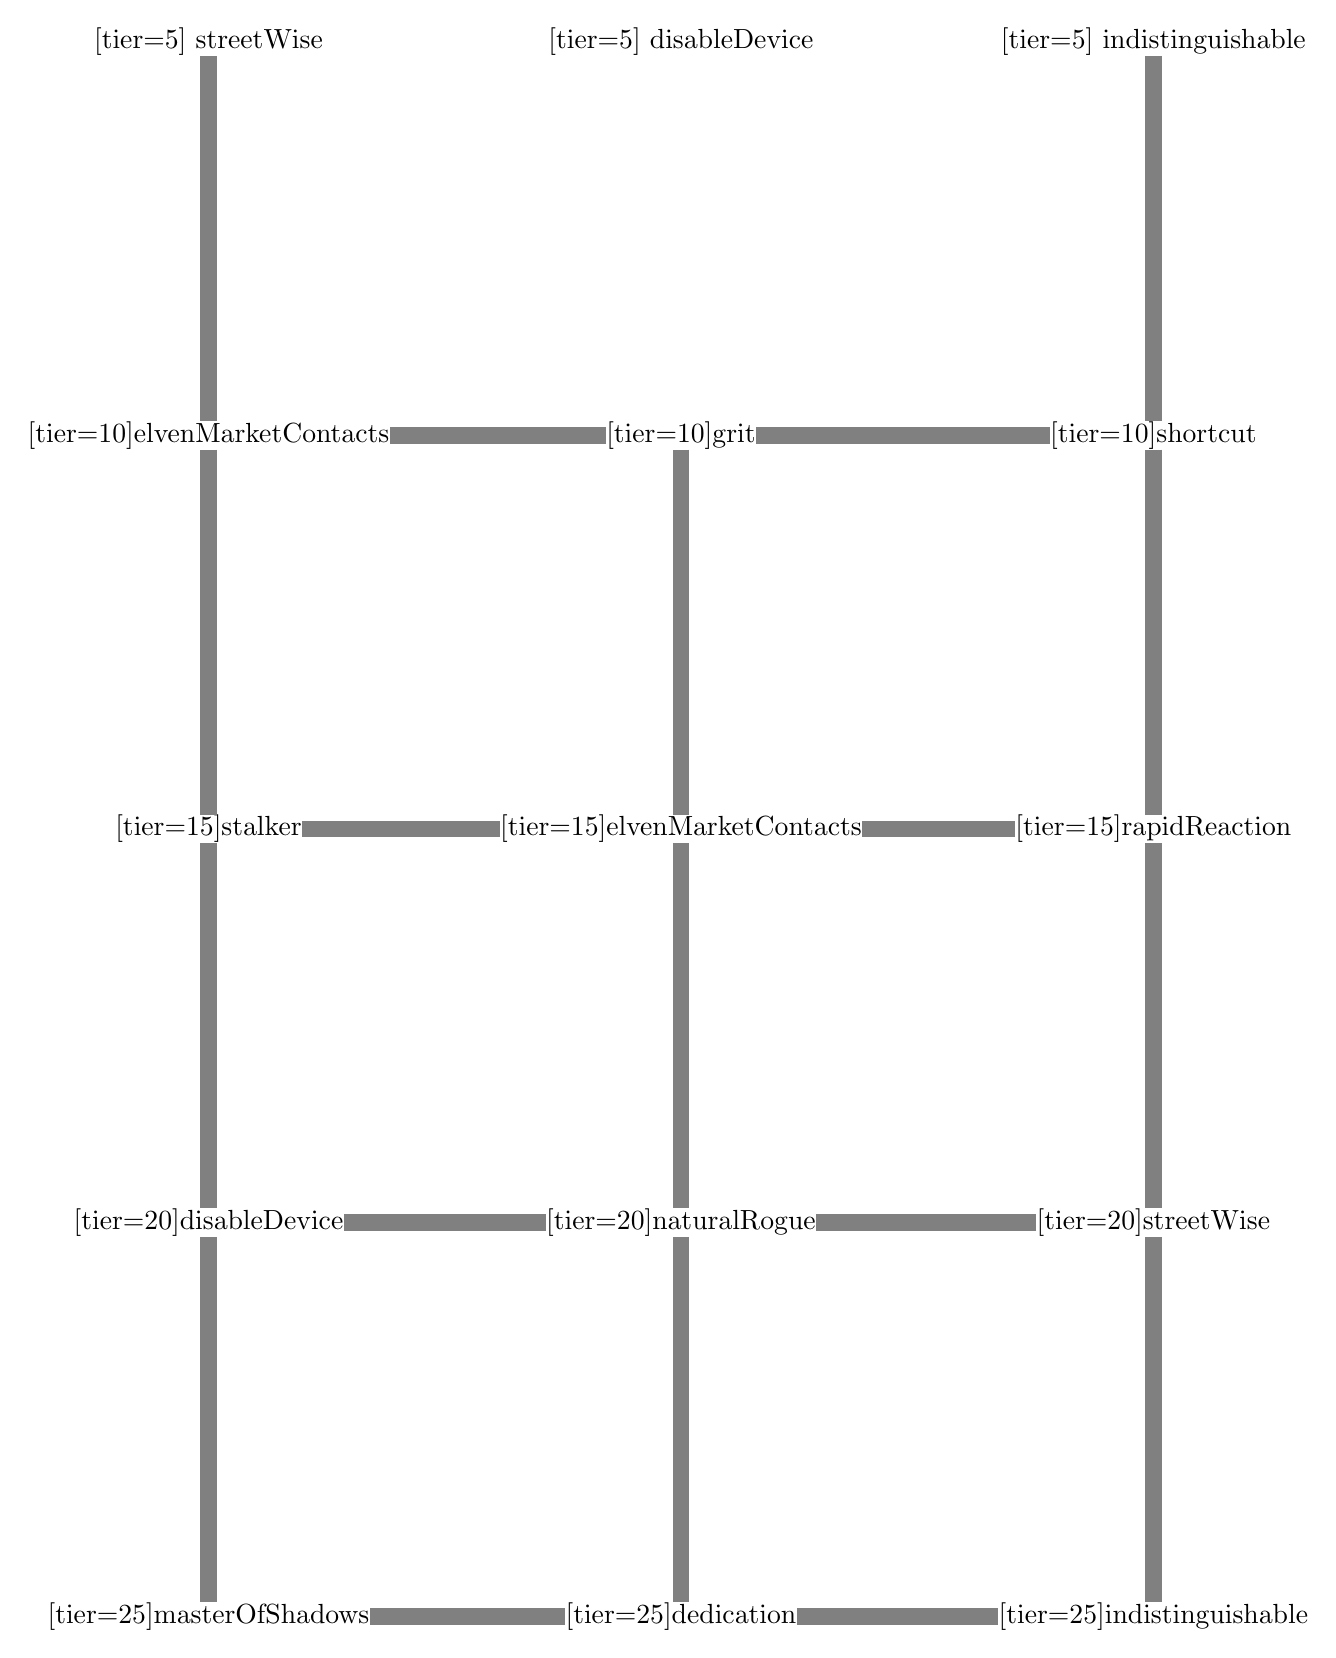
\begin{tikzpicture}
        \draw ( 0,  0) node(aa)[inner sep=0]{\TalentBox[tier=5] {streetWise}}
              ( 6,  0) node(ab)[inner sep=0]{\TalentBox[tier=5] {disableDevice}}
              (12,  0) node(ac)[inner sep=0]{\TalentBox[tier=5] {indistinguishable}}
              ( 0, -5) node(ba)[inner sep=0]{\TalentBox[tier=10]{elvenMarketContacts}}
              ( 6, -5) node(bb)[inner sep=0]{\TalentBox[tier=10]{grit}}
              (12, -5) node(bc)[inner sep=0]{\TalentBox[tier=10]{shortcut}}
              ( 0,-10) node(ca)[inner sep=0]{\TalentBox[tier=15]{stalker}}
              ( 6,-10) node(cb)[inner sep=0]{\TalentBox[tier=15]{elvenMarketContacts}}
              (12,-10) node(cc)[inner sep=0]{\TalentBox[tier=15]{rapidReaction}}
              ( 0,-15) node(da)[inner sep=0]{\TalentBox[tier=20]{disableDevice}}
              ( 6,-15) node(db)[inner sep=0]{\TalentBox[tier=20]{naturalRogue}}
              (12,-15) node(dc)[inner sep=0]{\TalentBox[tier=20]{streetWise}}
              ( 0,-20) node(ea)[inner sep=0]{\TalentBox[tier=25]{masterOfShadows}}
              ( 6,-20) node(eb)[inner sep=0]{\TalentBox[tier=25]{dedication}}
              (12,-20) node(ec)[inner sep=0]{\TalentBox[tier=25]{indistinguishable}}
        ;

        \tikzstyle{bar}=[gray,-,>=stealth, line width=6pt]

        \draw [bar] (aa) to (ba);
        \draw [bar] (ac) to (bc);
        \draw [bar] (ba) to (ca);
        \draw [bar] (bb) to (cb);
        \draw [bar] (bc) to (cc);
        \draw [bar] (ca) to (da);
        \draw [bar] (cb) to (db);
        \draw [bar] (cc) to (dc);
        \draw [bar] (da) to (ea);
        \draw [bar] (db) to (eb);
        \draw [bar] (dc) to (ec);

        \draw [bar] (ba) to (bb);
        \draw [bar] (bc) to (bb);

        \draw [bar] (ca) to (cb);
        \draw [bar] (cc) to (cb);

        \draw [bar] (da) to (db);
        \draw [bar] (dc) to (db);

        \draw [bar] (ea) to (eb);
        \draw [bar] (ec) to (eb);
    \end{tikzpicture}
}

\newcommand{\thugDescription}{
\section{Thug}
\epigraph{\textit{
    "thug quote"
} }{
    thug quotee
}
    Some Description
    \\
    See \nref{tlttree:thug} for more information.
}

\newcommand{\thugTree}{
    \newpage
    \subsection{Thug Talent Tree}
    \label{tlttree:thug}

    \textbf{Class Skills:} Coercion, Streetwise, Knowledge (Underworld), Brawl
    \newline

    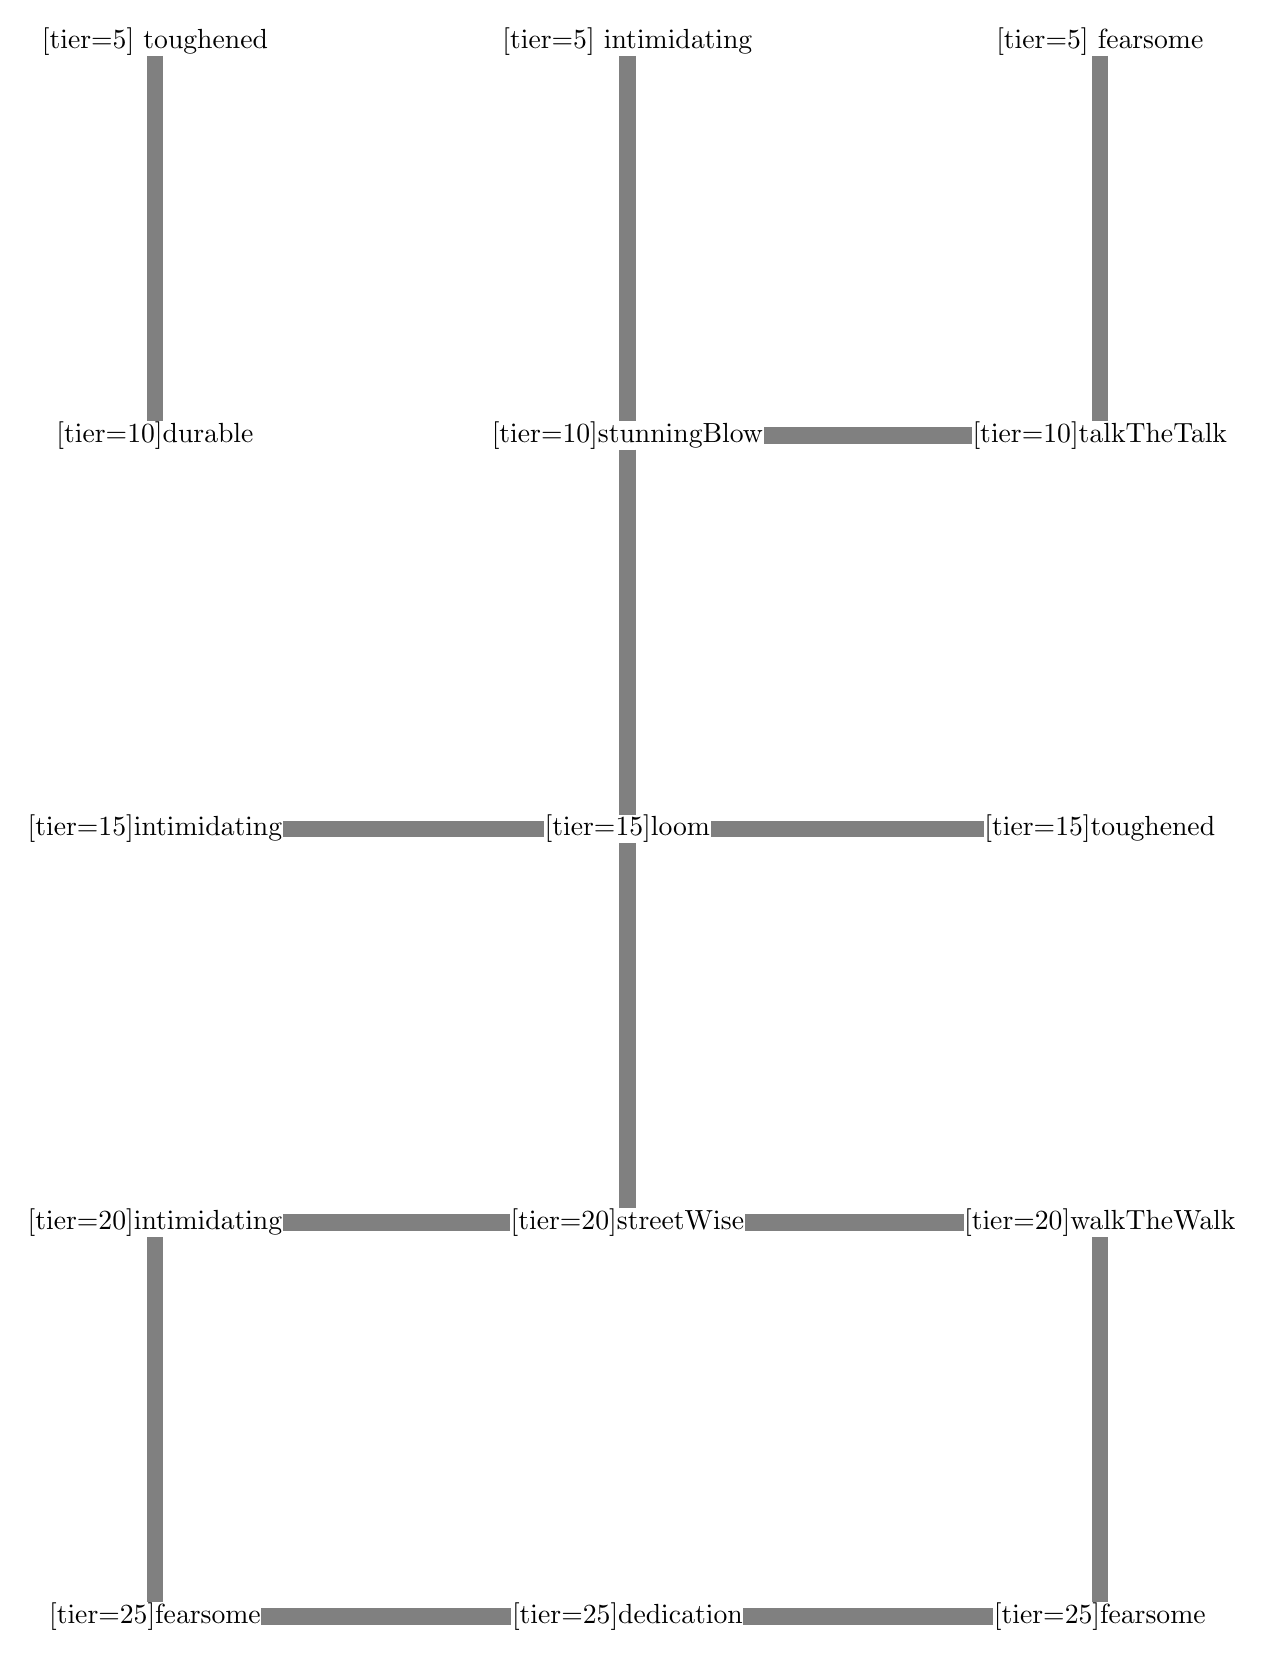
\begin{tikzpicture}
        \draw ( 0,  0) node(aa)[inner sep=0]{\TalentBox[tier=5] {toughened}}
              ( 6,  0) node(ab)[inner sep=0]{\TalentBox[tier=5] {intimidating}}
              (12,  0) node(ac)[inner sep=0]{\TalentBox[tier=5] {fearsome}}
              ( 0, -5) node(ba)[inner sep=0]{\TalentBox[tier=10]{durable}}
              ( 6, -5) node(bb)[inner sep=0]{\TalentBox[tier=10]{stunningBlow}}
              (12, -5) node(bc)[inner sep=0]{\TalentBox[tier=10]{talkTheTalk}}
              ( 0,-10) node(ca)[inner sep=0]{\TalentBox[tier=15]{intimidating}}
              ( 6,-10) node(cb)[inner sep=0]{\TalentBox[tier=15]{loom}}
              (12,-10) node(cc)[inner sep=0]{\TalentBox[tier=15]{toughened}}
              ( 0,-15) node(da)[inner sep=0]{\TalentBox[tier=20]{intimidating}}
              ( 6,-15) node(db)[inner sep=0]{\TalentBox[tier=20]{streetWise}}
              (12,-15) node(dc)[inner sep=0]{\TalentBox[tier=20]{walkTheWalk}}
              ( 0,-20) node(ea)[inner sep=0]{\TalentBox[tier=25]{fearsome}}
              ( 6,-20) node(eb)[inner sep=0]{\TalentBox[tier=25]{dedication}}
              (12,-20) node(ec)[inner sep=0]{\TalentBox[tier=25]{fearsome}}
        ;

        \tikzstyle{bar}=[gray,-,>=stealth, line width=6pt]

        \draw [bar] (aa) to (ba);
        \draw [bar] (ab) to (bb);
        \draw [bar] (ac) to (bc);

        \draw [bar] (bb) to (cb);

        \draw [bar] (cb) to (db);

        \draw [bar] (da) to (ea);
        \draw [bar] (dc) to (ec);

        \draw [bar] (bc) to (bb);

        \draw [bar] (ca) to (cb);
        \draw [bar] (cc) to (cb);

        \draw [bar] (da) to (db);
        \draw [bar] (dc) to (db);

        \draw [bar] (ea) to (eb);
        \draw [bar] (ec) to (eb);
    \end{tikzpicture}
}


\chapter{Specialisations}\label{chap:specs}

\epigraph{\textit{
"There are many paths to power, but all power comes at a price. Fame or infamy follows those who make great sacrifices
and who reach grand achievements. Would you be called tyrant or savior, I wonder. Perhaps you would prefer to be
addressed as Mighty One, or plain and simply by your birthname? Will the bards speak of you as delusional or
omnipotent? It all depends on the eye that sees. The hero of one is villain to another. But all beings of power share one
trait -each has its own secrets. Remnants of the past, stories of the now, or visions of the future - secrets are the source of
power. And the keepers of the greatest secrets are the most dangerous of all beings, for they will use any means to prevent
others from unveiling them." } } { The Oracle, Blue Shrine Scrolls }

As stated in ~\chapterref{creation} Each character combined two specialisations to form his or her career. In addition, it is
possible to buy new careers using experience points as mentioned in ~\tableref{experience}.

\begin{multicols}{2}

\ambassadorDescription
\arcanaDescription
\archerDescription
\assassinDescription
\beastRiderDescription
\gameHunterDescription
%\bodyguardDescription
\charmerDescription
%\con_artistDescription
\duneTraderDescription
\gladiatorDescription
\mercenaryDescription
%\nomadDescription
\performerDescription
\doctorDescription
\primalDescription
\psionDescription
%\raiderDescription
\scholarDescription
\scoutDescription
%\soulBladeDescription
\thiefDescription
\thugDescription

\end{multicols}

\section{Talent Trees}

\ambassadorTree
\arcanaTree
\archerTree
\assassinTree
\beastRiderTree
\gameHunterTree
%\bodyguardTree
\charmerTree
%\con_artistTree
\duneTraderTree
\gladiatorTree
\mercenaryTree
%\nomadTree
\performerTree
\doctorTree
\primalTree
\psionTree
%\raiderTree
\scholarTree
\scoutTree
%\soulBladeTree
\thiefTree
\thugTree
